% ******************************* PhD Thesis Template **************************
% Please have a look at the README.md file for info on how to use the template

\documentclass[a4paper,12pt,times,numbered,print,index]{Classes/PhDThesisPSnPDF}
% \documentclass[a4paper,12pt,twoside,openright]{report}

% ******************************************************************************
% ******************************* Class Options ********************************
% *********************** See README for more details **************************
% ******************************************************************************

% `a4paper'(The University of Cambridge PhD thesis guidelines recommends a page
% size a4 - default option) or `a5paper': A5 Paper size is also allowed as per
% the Cambridge University Engineering Deparment guidelines for PhD thesis
%
% `11pt' or `12pt'(default): Font Size 10pt is NOT recommended by the University
% guidelines
%
% `oneside' or `twoside'(default): Printing double side (twoside) or single
% side.
%
% `print': Use `print' for print version with appropriate margins and page
% layout. Leaving the options field blank will activate Online version.
%
% `index': For index at the end of the thesis
%
% `draftclassic': For draft mode without loading any images (same as draft in book)
%
% `draft': Special draft mode with line numbers, images, and water mark with
% timestamp and custom text. Position of the text can also be modified.
%
% `abstract': To generate only the title page and abstract page with
% dissertation title and name, to submit to the Student Registry
%
% `chapter`: This option enables only the specified chapter and it's references
%  Useful for review and corrections.
%
% ************************* Custom Page Margins ********************************
%
% `custommargin`: Use `custommargin' in options to activate custom page margins,
% which can be defined in the preamble.tex. Custom margin will override
% print/online margin setup.
%
% *********************** Choosing the Fonts in Class Options ******************
%
% `times' : Times font with math support. (The Cambridge University guidelines
% recommend using times)
%
% `fourier': Utopia Font with Fourier Math font (Font has to be installed)
%            It's a free font.
%
% `customfont': Use `customfont' option in the document class and load the
% package in the preamble.tex
%
% default or leave empty: `Latin Modern' font will be loaded.
%
% ********************** Choosing the Bibliography style ***********************
%
% `authoryear': For author-year citation eg., Krishna (2013)
%
% `numbered': (Default Option) For numbered and sorted citation e.g., [1,5,2]
%
% `custombib': Define your own bibliography style in the `preamble.tex' file.
%              `\RequirePackage[square, sort, numbers, authoryear]{natbib}'.
%              This can be also used to load biblatex instead of natbib
%              (See Preamble)
%
% **************************** Choosing the Page Style *************************
%
% `default (leave empty)': For Page Numbers in Header (Left Even, Right Odd) and
% Chapter Name in Header (Right Even) and Section Name (Left Odd). Blank Footer.
%
% `PageStyleI': Chapter Name next & Page Number on Even Side (Left Even).
% Section Name & Page Number in Header on Odd Side (Right Odd). Footer is empty.
%
% `PageStyleII': Chapter Name on Even Side (Left Even) in Header. Section Number
% and Section Name in Header on Odd Side (Right Odd). Page numbering in footer

% Uncomment to change page style
%\pagestyle{PageStyleII}

% ********************************** Preamble **********************************
% Preamble: Contains packages and user-defined commands and settings
% ******************************************************************************
% ****************************** Custom Margin *********************************

% Add `custommargin' in the document class options to use this section
% Set {innerside margin / outerside margin / topmargin / bottom margin}  and
% other page dimensions
\ifsetCustomMargin
  \RequirePackage[left=37mm,right=30mm,top=35mm,bottom=30mm]{geometry}
  \setFancyHdr % To apply fancy header after geometry package is loaded
\fi

% Add spaces between paragraphs
%\setlength{\parskip}{0.5em}
% Ragged bottom avoids extra whitespaces between paragraphs
\raggedbottom
% To remove the excess top spacing for enumeration, list and description
%\usepackage{enumitem}
%\setlist[enumerate,itemize,description]{topsep=0em}

% *****************************************************************************
% ******************* Fonts (like different typewriter fonts etc.)*************

% Add `customfont' in the document class option to use this section

\ifsetCustomFont
  % Set your custom font here and use `customfont' in options. Leave empty to
  % load computer modern font (default LaTeX font).
  \RequirePackage{helvet}

  % For use with XeLaTeX
    \setmainfont[
      Path              = ./libertine/opentype/,
      Extension         = .otf,
      UprightFont = LinLibertine_R,
      BoldFont = LinLibertine_RZ, % Linux Libertine O Regular Semibold
      ItalicFont = LinLibertine_RI,
      BoldItalicFont = LinLibertine_RZI, % Linux Libertine O Regular Semibold Italic
   ]
   {libertine}
  %  % load font from system font
  \newfontfamily\libertinesystemfont{Linux Libertine O}
\fi

% *****************************************************************************
% **************************** Custom Packages ********************************

% ************************* Algorithms and Pseudocode **************************

%\usepackage{algpseudocode}


% ********************Captions and Hyperreferencing / URL **********************

% Captions: This makes captions of figures use a boldfaced small font.
%\RequirePackage[small,bf]{caption}

\RequirePackage[labelsep=space,tableposition=top]{caption}
\renewcommand{\figurename}{Fig.} %to support older versions of captions.sty


% *************************** Graphics and figures *****************************

%\usepackage{rotating}
%\usepackage{wrapfig}

% Uncomment the following two lines to force Latex to place the figure.
% Use [H] when including graphics. Note 'H' instead of 'h'
%\usepackage{float}
%\restylefloat{figure}

% Subcaption package is also available in the sty folder you can use that by
% uncommenting the following line
% This is for people stuck with older versions of texlive
%\usepackage{sty/caption/subcaption}
\usepackage{graphicx}
\usepackage{subcaption}
%\usepackage{subfig}

% ********************************** Tables ************************************
\usepackage{booktabs} % For professional looking tables
\usepackage{multirow}
\usepackage{mathtools}
\usepackage{algorithm}
\usepackage{algorithmic}

%% \usepackage{algorithmicx}

%\usepackage{multicol}
%\usepackage{longtable}
%\usepackage{tabularx}



% *********************************** SI Units *********************************
\usepackage{siunitx} % use this package module for SI units


% ******************************* Line Spacing *********************************

% Choose linespacing as appropriate. Default is one-half line spacing as per the
% University guidelines

% \doublespacing
% \onehalfspacing
% \singlespacing


% ************************ Formatting / Footnote *******************************

% Don't break enumeration (etc.) across pages in an ugly manner (default 10000)
%\clubpenalty=500
%\widowpenalty=500

%\usepackage[perpage]{footmisc} %Range of footnote options


% *****************************************************************************
% *************************** Bibliography  and References ********************

%\usepackage{cleveref} %Referencing without need to explicitly state fig /table

% Add `custombib' in the document class option to use this section
\ifuseCustomBib
   \RequirePackage[square, sort, numbers, authoryear]{natbib} % CustomBib

% If you would like to use biblatex for your reference management, as opposed to the default `natbibpackage` pass the option `custombib` in the document class. Comment out the previous line to make sure you don't load the natbib package. Uncomment the following lines and specify the location of references.bib file

%\RequirePackage[backend=biber, style=numeric-comp, citestyle=numeric, sorting=nty, natbib=true]{biblatex}
%\bibliography{References/references} %Location of references.bib only for biblatex

\fi

% changes the default name `Bibliography` -> `References'
\renewcommand{\bibname}{References}


% ******************************************************************************
% ************************* User Defined Commands ******************************
% ******************************************************************************

% *********** To change the name of Table of Contents / LOF and LOT ************

%\renewcommand{\contentsname}{My Table of Contents}
%\renewcommand{\listfigurename}{My List of Figures}
%\renewcommand{\listtablename}{My List of Tables}


% ********************** TOC depth and numbering depth *************************

\setcounter{secnumdepth}{2}
\setcounter{tocdepth}{2}


% ******************************* Nomenclature *********************************

% To change the name of the Nomenclature section, uncomment the following line

%\renewcommand{\nomname}{Symbols}


% ********************************* Appendix ***********************************

% The default value of both \appendixtocname and \appendixpagename is `Appendices'. These names can all be changed via:

%\renewcommand{\appendixtocname}{List of appendices}
%\renewcommand{\appendixname}{Appndx}

% *********************** Configure Draft Mode **********************************

% Uncomment to disable figures in `draft'
%\setkeys{Gin}{draft=true}  % set draft to false to enable figures in `draft'

% These options are active only during the draft mode
% Default text is "Draft"
%\SetDraftText{DRAFT}

% Default Watermark location is top. Location (top/bottom)
%\SetDraftWMPosition{bottom}

% Draft Version - default is v1.0
%\SetDraftVersion{v1.1}

% Draft Text grayscale value (should be between 0-black and 1-white)
% Default value is 0.75
%\SetDraftGrayScale{0.8}


% ******************************** Todo Notes **********************************
%% Uncomment the following lines to have todonotes.

%\ifsetDraft
%	\usepackage[colorinlistoftodos]{todonotes}
%	\newcommand{\mynote}[1]{\todo[author=kks32,size=\small,inline,color=green!40]{#1}}
%\else
%	\newcommand{\mynote}[1]{}
%	\newcommand{\listoftodos}{}
%\fi

% Example todo: \mynote{Hey! I have a note}

% ************************ Thesis Information & Meta-data **********************
% Thesis title and author information, refernce file for biblatex
% ************************ Thesis Information & Meta-data **********************
%% The title of the thesis
\title{Parameter Optimization using high-dimensional Bayesian Optimization}
%\texorpdfstring is used for PDF metadata. Usage:
%\texorpdfstring{LaTeX_Version}{PDF Version (non-latex)} eg.,
%\texorpdfstring{$sigma$}{sigma}

%% Subtitle (Optional)
\subtitle{Bachelor Thesis}

%% The full name of the author
\author{David Yenicelik}

%% Department (eg. Department of Engineering, Maths, Physics)
\dept{Department of Computer Science}

%% University and Crest
\university{Swiss Federal Institute of Technology in Zurich}
% Crest minimum should be 30mm.
\crest{
\includegraphics[width=0.5\textwidth]{University_Crest}}
%% Use this crest, if you are using the college crest
%% Crest long miminum should be 65mm
%\crest{
\includegraphics[width=0.45\textwidth]{University_Crest_Long}}

%% College shield [optional] 
% Crest minimum should be 30mm.
%\collegeshield{
\includegraphics[width=0.2\textwidth]{CollegeShields/Kings}}


%% Supervisor (optional)
%% for multiple supervisors, append each supervisor with the \newline command
%\supervisor{Prof. A.B. Supervisor\newline
%Prof. C.D. Supervisor}

%% Supervisor Role (optional) - Supervisor (default) or advisor
% \supervisorrole{\textbf{Supervisors: }}
%% if no title is desired:
% \supervisorrole{}

%% Supervisor line width: required to align supervisors
%\supervisorlinewidth{0.35\textwidth}

%% Advisor (optional)
%% for multiple advisors, append each advisor with the \newline command
%\advisor{Dr. A. Advisor\newline
%Dr. B. Advisor}
     
%% Advisor Role (optional) - Advisor (default) or leave empty
% \advisorrole{Advisors: }
%% if no title is required
% \advisorrole{}

%% Advisor line width: required to align supervisors
%\advisorlinewidth{0.25\textwidth}


%% You can redefine the submission text:
% Default as per the University guidelines:
% ``''
%\renewcommand{\submissiontext}{change the default text here if needed}
% This dissertation is submitted for the degree of

%% Full title of the Degree
%\degreetitle{Doctor of Philosophy}

%% College affiliation (optional)
%\college{King's College}

%% Submission date
% Default is set as {\monthname[\the\month]\space\the\year}
%\degreedate{September 2014} 

%% Meta information
\subject{LaTeX} \keywords{{LaTeX} {PhD Thesis} {Engineering} {University of
Cambridge}}


% ***************************** Abstract Separate ******************************
% To printout only the titlepage and the abstract with the PhD title and the
% author name for submission to the Student Registry, use the `abstract' option in
% the document class.

\ifdefineAbstract
 \pagestyle{empty}
 \includeonly{Declaration/declaration, Abstract/abstract}
\fi

% ***************************** Chapter Mode ***********************************
% The chapter mode allows user to only print particular chapters with references
% Title, Contents, Frontmatter are disabled by default
% Useful option to review a particular chapter or to send it to supervisior.
% To use choose `chapter' option in the document class

\ifdefineChapter
 \includeonly{Chapter3/chapter3}
\fi

% ******************************** Front Matter ********************************
\begin{document}

\frontmatter

\maketitle

%% Abstract
% ************************** Thesis Abstract *****************************
% Use `abstract' as an option in the document class to print only the titlepage and the abstract.
\begin{abstract}

In this thesis, I explore the possibilities of conducting bayesian optimization techniques in high dimensional domains.
Although high dimensional domains can be defined to be between hundreds and thousands of dimensions, we will primarily focus on problem settings that occur between two and 20 dimensions.
As such, we focus on solutions to practical problems, such as tuning the parameters for an electron accelerator, or for even simpler tasks that can be run and optimizated just in time with a common laptop at hand. \\

I follow a systematic methodology, where we identify problems currently occurring with Bayesian Optimization methods.
For this, I take on the following steps: \\

I first provide a theoretic background to the mathematical foundations of Gaussian Processes at hand.
I present the derivation of the surrogate functions as a foundation to better understand what parts of the process can be optimized.
I then shortly discuss the different acquisition functions that are most often used in practice.\\

I continue by exploring different techniques that are currently considered as state-of-the-art. 
Most of these techniques concentrate on doing one of three things.
The most common approach is to do a linear dimensionality reduction.
The second most common approach is to identify variables that rely on each other, and create different Gaussian Processes for each group of variables that depend on each other. \\

I identify the shortcomings of the current methods and present quantitative ways on how we can measure improvements for the goal at hand.
Together with my supervisors, we present a novel algorithm called "BORING" to do Bayesian Optimization at hand.
This algorithm combines the advantages of linear projection methods, but also allows to take into consideration some small perturbations in the target function.
Taking into account smaller perturbations is something that linear reduction models have not taken into account so far.
BORING proves to have all the advantages that other state-of-the-art linear dimensionality reduction algorithms have.
However, BORING improves this state by allowing small perturbations to be taken into account when creating the surrogate function. 
This feature ultimately allows BORING to be more accurate when modelling functions that we want to optimize over. \\

Finally, we evaluate BORING and compare it to the competitive state-of-the-art in Bayesian Optimization.
We do a quantitative analysis by applying the Gaussian Process algorithms on different, well defined functions and measuring the regret during optimization that it achieves.
We do a qualitative analysis by visualizing the predicted surrogate function, and comparing this to the real function.
In addition to that, we do a short experiment on whether the subspace identification method can be used to do feature selection, by choosing the projection in such a way, that the most important features will receive the highest matrix weights. \\

Our main contribution is BORING, an algorithm which is competitive with other state-of-the-art methods in Bayesian Optimization.
The main features of BORING are 1.) the possibility to identify the subspace (unlike most other optimization algorithms), and 2.) to provide a much lower penalty to identify the subspace, as optimization is still the main goal.

\end{abstract}


% *********************** Adding TOC and List of Figures ***********************

\tableofcontents

% \printnomenclature[space] space can be set as 2em between symbol and description
%\printnomenclature[3em]

\printnomenclature

% ******************************** Main Matter *********************************
\mainmatter
%% Introduction (to the structure of the work
% %!TEX root = ../thesis.tex
%*******************************************************************************
%*********************************** First Chapter *****************************
%*******************************************************************************

\chapter{Background}  %Title of the First Chapter

\ifpdf
    \graphicspath{{Chapter1/Figs/Raster/}{Chapter1/Figs/PDF/}{Chapter1/Figs/}}
\else
    \graphicspath{{Chapter1/Figs/Vector/}{Chapter1/Figs/}}
\fi


%********************************** %First Section  **************************************
\section{Bayesian Optimization in high dimensions} %Section - 1.1 

Many of today's problems can be boiled down to some flavor of black box optimization. 
Such problems include neural architecture search, hyper-parameter search for neural networks, parameter optimization for electron accelerators, or drone parameter optimization using safety constraints (CITE Johannes). \\

Bayesian optimization methods are a class of sequential black-box optimization methods, where we learn a surrogate function surface using a Gaussian prior, and a Gaussian likelihood function.
Combining the prior and the likelihood results in the Gaussian Posterior, which we then can be used as a surface over which we try to optimize. \\

Bayesian optimization is a method that has increasingly gained attention in the last decades, as it requires relatively few points to find an appropriate response surface for the function over which we want to optimize over.
It is a sequential model based optimization function, which means that we choose the best point $x^*_i$ given all previous points $x^*_{i-1}, x^*_{i-2}, \ldots, x^*_{0}$.
Given certain acquisition functions, it offers a good mixture of exploration and exploitation from an empirical standpoint. \\

Bayesian optimization is a method that has increasingly gained success in finding a good mixture between exploration the search space (finding new hyper-parameter configurations that outperform all existing configurations), and exploiting currently found best configurations (using the best learned hyper-parameter configurations to get utility out of the system). \\

However, as machine learning algorithms and other problems become more complex, Bayesian optimization needs to cope with the increasing number of dimensions that define the search space of possible configurations.
Because BO methods loose effectiveness in higher dimensions, this work deals with methods that work in higher dimensions.

\section{Gaussian Processes}
In Bayesian Optimization, we want to use a Gaussian Process to find an optimal parameter setting $\mathbf{x^*}$ that maximizes a given utility function $f$.
We assume the response surface to be Lipschitz-continuous. \\

Assume we have observations $ \mathcal{Y} = \{ y^{(1)}, \ldots, y^{(N)} \}$, each evaluated at a point $ \mathcal{X} = \{  \mathbf{x}^{(1)}, \ldots, \mathbf{x}^{(N)} \}$.
The relationship between the observations $y$ and individual parameter settings $\mathbf{x}$ is $y = f \left( \mathbf{x} \right) + \epsilon$ where $\epsilon \sim  \mathcal{N} \left( 0, \sigma^2_n \right)$. Any quantity to be predicted has a subscript-star (e.g. $y_*$ is the function evaluation we want to predict).\\

In it's simplest form, a Gaussian Process is described by the following equation:

\begin{equation}
\begin{pmatrix} y \\
y_* \end{pmatrix} \sim N\Biggl(\mu,\begin{pmatrix} K & K^T_*\\
 K_* & K_{**} \end{pmatrix}\Biggr),
\end{equation}

Where $\mu$ is a mean function, $K = \text{kernel}(\mathbf{X}, \mathbf{X})$, $K_* = \text{kernel}(\mathbf{x_*}, \mathbf{X})$ and $K_{**} = \text{kernel}(\mathbf{x_*}, \mathbf{x_*})$.
We predict any new point $y_*$, (given all previously sampled points $y$) by estimating the probability $ p(y_*|y) \sim N(K_*K^{-1}y,K_{**}-K_*K^{-1}K'_*) $

This, in turn, can be used to build an acquisition function. 
This acquisition function describes where to best sample points next.
Some popular acquisition functions include GP-UCB, Most probable improvement (MPI) and Expected Improvement (EI).
The choice of the acquisition function has significant influence on the performance of the optimization procedure.\\

We will talk about the problems and possible solutions for the task at hand in the next section.

\subsection{Derivation of the Gaussian Process Formula}
The prior for the Gaussian Process it the following (assuming a 0-mean-prior).

\begin{equation}
u \sim GP(0, k(x, x'))
\end{equation}

Because $u$ is a random variable, it's probably distribution is given by a normal distribution (as determined by the Gaussian Process):

\begin{equation}
p(u) = N ( 0, K )
\end{equation}

Now we go over to observing some data $ X = \{ (x_1, y_1), \ldots, (x_n, y_n) \} $ where $y$ has some noise term $\epsilon$ such that $y = u(x) + \epsilon$.
We assume that $\epsilon$ is normally distributed around $0$ with $\sigma$ standard deviation.
This means that the likelihood takes on the following form:

\begin{equation}
p(y | x, u) = N (u, \sigma^2 I)
\end{equation}

% https://stats.stackexchange.com/questions/84058/derivation-of-predictive-distribution-of-gaussian-process

Now we want to derive the posterior of the Gaussian Process, given the likelihood and the prior.
We use Bayes rule to derive this.

\begin{align}
p(u | x, y) &= \frac{ p(y | x, u) p(u) }{p(y | x)}
& = N( K(K +\sigma^2 I)^{-1}y, \sigma^2 (K + \sigma^2 I)^{-1} K )
\end{align}

At this point, we want to create a surrogate embedding, which predicts $y_*$ for any possible given $x_*$. 
We refer to this as the surrogate response surface.

We use the following formula to derive the posterior distribution for a given predictor $y_*$.

\begin{equation}
\begin{pmatrix} y \\
y_* \end{pmatrix} \sim N\Biggl(\mu,\begin{pmatrix} K & K^T_*\\
 K_* & K_{**} \end{pmatrix}\Biggr),
\end{equation}

To numerically calculate this, one uses the Matrix Inversion Lemma (CITE Murphy Chapter 4.3 110-111)


\section{Acquisition Functions}

Given the above formula for the posterior mean $\mu$ and the poster variance $\sigma^2$, Bayesian Optimization uses an acquisition function to optimize over.
We quickly present some of the most common acquisition functions.

% Most formulae taken from "A tutorial on Bayesian optimization of expensive cost functions, with application to active user modeling and hierarchical reinforcement learning

\subsection{Upper Confident Bound (UCB)}
(CITE Krause Srinivas) about how acquisition function is guaranteed to find the best config after awhile.

The upper confidence bound allows the user to control exploitation and exploration through a parameter $\beta > 0$, which can be chosen as CITE PAPER, to offer optimality guarantees.

\begin{equation}
UCB(x) = \mu(x) + \beta \sigma(x)
\end{equation}

Here, the functions $\mu$ and $\sigma$ are the predicted mean and variance of the Gaussian Process Posterior.

\subsection{Probability of Improvement (PI)}
The (maximum) probability of improvement always selects the point which has the highest potential to maximize the function. 
The downside to this policy is that this leads to exploitation, which can be controlled by a parameter $\xi > 0$.

\begin{align}
    PI(x) & = P( f(x) \geq f(x^+) + \xi ) \\
    & = \Phi ( \frac{\mu(x) - f(x^+) - \xi}{\sigma(x)}  ) 
\end{align}


\subsection{Expected Improvement (EI)}

"CITE A tutorial on Bayesian optimization of expensive cost functions, with application to active user modeling and hierarchical reinforcement learning."
\begin{align}
    EI(x) =
    \begin{dcases}
        ( \mu (x) - f(x^+) \Phi(Z) \sigma (x) \phi (Z) ) & \text{ if } \sigma (x) > 0 \\
        0 & \text{ if } \sigma (x) = 0
    \end{dcases} \\
\end{align}

\begin{equation}
    Z = \frac{\mu (x) - f(x^+) }{\sigma(x)}
\end{equation}

Given one of the above acquisition functions, we then use an optimizer such as $L-BFGS$, to find an approximate global maximum of the respective function.
The combination of Gaussian Processes and Acquisition function together result in a Bayesian Optimization algorithm, which has a prior assumption about the function to be learned and uses data samples to create a likelihood to refine the posterior of the function assumption further.

\section{Resources}
(CITE https://github.com/SheffieldML/GPy)
We will use "GPy: A Gaussian process framework in python" and "CITE https://github.com/SheffieldML/GPyOpt" by the Sheffield Machine Learning Group.
In addition to that, the febo framework developed by Johannes Kirschner from the Learning and Adaptive Systems group at ETH Zurich.
We use pytest to write tests (CITE).

% BFGS: https://stats.stackexchange.com/questions/284712/how-does-the-l-bfgs-work

%% Introduction
% ************************** Thesis Abstract *****************************
% Use `abstract' as an option in the document class to print only the titlepage and the abstract.
\chapter{Introduction}
\subsection{Motivation}

Tuning hyperparameters is considered a computationally intensive and tedious task, be it for neural networks, or complex physical instruments such as free electron lasers.
Users for such applications could benefit from a 'one-click-search' feature, which would find optimal parameters in as few function evaluations as possible.
This project aims to find such an algorithm which is both efficient and holds certain convergence guarantees.
We focus our efforts on Bayesian Optimization (BO) and revise techniques for high-dimensional BO. \\

\subsection{Background}

In Bayesian Optimization, we want to use a Gaussian Process to find an optimal parameter setting $\mathbf{x^*}$ that maximizes a given utility function $f$.
We assume the response surface to be Lipschitz-continuous. \\

Assume we have observations $ \mathcal{Y} = \{ y^{(1)}, \ldots, y^{(N)} \}$, each evaluated at a point $ \mathcal{X} = \{  \mathbf{x}^{(1)}, \ldots, \mathbf{x}^{(N)} \}$.
The relationship between the observations $y$ and individual parameter settings $\mathbf{x}$ is $y = f \left( \mathbf{x} \right) + \epsilon$ where $\epsilon \sim  \mathcal{N} \left( 0, \sigma^2_n \right)$. Any quantity to be predicted has a subscript-star (e.g. $y_*$ is the function evaluation we want to predict).\\

In it's simplest form, a Gaussian Process is described by the following equation:

\begin{equation}
\begin{pmatrix} y \\
y_* \end{pmatrix} \sim N\Biggl(\mu,\begin{pmatrix} K & K^T_*\\
 K_* & K_{**} \end{pmatrix}\Biggr),
\end{equation}

Where $\mu$ is a mean function, $K = \text{kernel}(\mathbf{X}, \mathbf{X})$, $K_* = \text{kernel}(\mathbf{x_*}, \mathbf{X})$ and $K_{**} = \text{kernel}(\mathbf{x_*}, \mathbf{x_*})$.
We predict any new point $y_*$, (given all previously sampled points $y$) by estimating the probability $ p(y_*|y) \sim N(K_*K^{-1}y,K_{**}-K_*K^{-1}K'_*) $

This, in turn, can be used to build an acquisition function. 
This acquisition function describes where to best sample points next.
Some popular acquisition functions include GP-UCB, Most probable improvement (MPI) and Expected Improvement (EI).
The choice of the acquisition function has great influence on the performance of the optimization procedure.\\

We will talk about the problems and possible solutions for the task at hand in the next section.

\subsection{Scope of the Project}

Bayesian optimization suffers from the curse of dimensionality. 
The goal of this project is to arrive at a solution that resolves the curse of dimensionality for the specific task with regards to Bayesian optimization.
This project includes, but is not limited to the following methods.\\

\begin{enumerate}
\item \cite{Tripathy}
Assume $f(x) \approx g( \mathbf{W}^T x)$ where $ \mathbf{W} \in \mathbb{R}^{D \times d} $ and $D >> d$.
We assume that $ \mathbf{W} $ is orthogonal as proposed in \cite{Tripathy}.

The algorithm does not require gradient-information (thus, easier to implement, and robust to noise).
The standard-deviation, kernel parameters and  $ \mathbf{W} $ can be found iteratively.
First we fix $ \mathbf{W} $, and optimize over the standard-deviation, kernel parameters.
Then we fix the standard-deviation, kernel parameters. and optimize over $ \mathbf{W} $.
We repeat this procedure until the change of the log-likelihood between iterations is below some $ \epsilon_l $.

\item \cite{Rolland}
Assume $f(x) = f^{(1)}( x^{(1)} )  + f^{(2)}( x^{(2)} ) + \ldots + f^{(M)}( x^{(M)} )$ where $ x^{(i)} \in \mathcal{X}^{(i)} \subseteq \mathcal{X}$, i.e. each function component  $f^{(i)}$ takes some lower-dimensional subspace as the input.
The lower-dimensional subspaces may overlap.
The mean and covariance of $f(x)$ is then the sum of the individual component's means and covariances.

An additive decomposition (as described above) can be represented by a dependency graph. The dependency graph is built by joining variables $i$ and $j$ with an edge whenever they appear together within some set $x(k)$. 

The goal is to maximize an acquisition function $ \phi_t(x) = \sum_{i=1}^M \phi_t^{(i)} ( x^{(i)} )$. 
This maximization is achieved by maximizing the probability of Markov Random Fields within the graph.
A junction tree is created from the graph, which is then used to find the global maximum of the acquisition function.

The dependencies between the variable-subsets are represented through a graph, which can be learned through Gibbs sampling.
This, in turn, is used to create a kernel for the GP.

% TODO: cite rembo!
\item \cite{Wang}
A function $f : \mathbf{R}^D \rightarrow \mathbf{R}$ is said to have effective dimensionality $d_e$ (where $d_e < D$), if there exists a linear subspace $\mathcal{T}$ of dimension $d_e$ such that for all $ x_\top \in \mathcal{T} \subset \mathbf{R}^D $ and $x_\perp \in \mathcal{T_\perp} \subset \mathbf{R}^D $, we have $ f(x) = f(x_\top +x_\perp ) = f(x_\top)$.
$\mathcal{T^\perp}$ is the orthogonal complement of $\mathcal{T}$.

Assume $ f : \mathbf{R}^D \rightarrow \mathbf{R} $ has effective dimensionality $d_e$.
Given a random matrix $ \mathbf{A} \in \mathbf{R}^{D \times d} $ (where $d \geq d_e$) with independent entries sampled fom $ \mathcal{N}(0, 1) $.
For any $ x \in \mathbf{R}^D $, there exists a $y \in \mathbf{R}^d $ such that $ f(x) = f(\mathbf{A} y ) $.
We now only need to optimize over all possible $y \in \mathbf{R}^d$, instead of all possible $x \in \mathbf{R}^D $.


\begin{figure}[h]
\centering
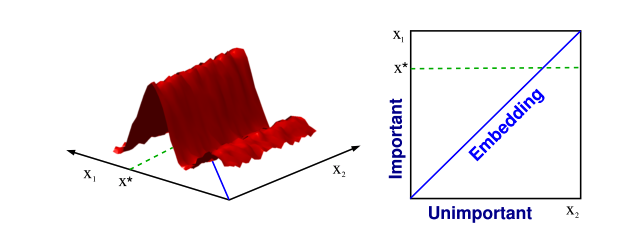
\includegraphics[width=0.5\textwidth]{./../src/Embedding_optimization.png}
\caption{ This function in D=2 dimesions only has d=1 effective dimension. Hence, the 1-dimensional embedding includes the 2-dimensional function’s optimizer. It is more efficient to search for the optimum along the 1-dimensional random embedding than in the original 2-dimensional space}
\end{figure}

\end{enumerate}

If, for some reason, finding an active subspace or an effective lower dimension is not possible, we are open to adapt the procedure of optimization.


%% Background
%!TEX root = ../thesis.tex
%*******************************************************************************
%*********************************** First Chapter *****************************
%*******************************************************************************

\chapter{Background}  %Title of the First Chapter

\ifpdf
    \graphicspath{{Chapter1/Figs/Raster/}{Chapter1/Figs/PDF/}{Chapter1/Figs/}}
\else
    \graphicspath{{Chapter1/Figs/Vector/}{Chapter1/Figs/}}
\fi


%********************************** %First Section  **************************************
\section{Bayesian Optimization in high dimensions} %Section - 1.1 

Many technical problems can be boiled down to some flavour of black box optimization. 
Such problems include neural architecture search \citep{BayesianOptimizationNAS}, hyper-parameter search for neural networks, parameter optimization for electron accelerators, or drone parameter optimization using safety constraints \citep{berkenkamp17saferl}. \\

Bayesian optimization methods are a class of sequential black box optimization methods.
A surrogate function surface is learned using a Gaussian prior, and a Gaussian likelihood function.
Combining the prior and the likelihood results in the Gaussian posterior, which can then be used as a surface over which optimization can take place, with the help of a chosen acquisition function. \\

Bayesian optimization is a method that has increasingly gained attention in the last decades, as it requires relatively few points to find an appropriate response surface for the function over which we want to optimize over.
It is a sequential model based optimization function, which means that we choose the best point $x^*_i$ given all previous points $x^*_{i-1}, x^*_{i-2}, \ldots, x^*_{0}$.
Given certain acquisition functions, it offers a good mixture between exploration and exploitation from an empirical standpoint \citep{BOIncreasingPopularityEmpirically}. \\

However, as machine learning algorithms, and other problems become more complex, Bayesian optimization needs to cope with the increasing number of dimensions that define the search space of possible configurations.
Because BO methods lose effectiveness in higher dimensions due to the curse of dimensionality, this work  explores Bayesian optimization methods that improve the optimization performance in higher dimensions.
Finally, we propose a novel method that can take into consideration small perturbations of the function we want to optimize over.

\section{Gaussian Processes}
Bayesian Optimization (BO) aims at using a Gaussian Process as an intermediate representation to find an optimal parameter setting $\mathbf{x^*}$ that maximizes a given utility function $f$.\\

Assume we have observations $ \mathcal{Y} = \{ y^{(1)}, \ldots, y^{(N)} \}$, each evaluated at a point $ \mathcal{X} = \{  \mathbf{x}^{(1)}, \ldots, \mathbf{x}^{(N)} \}$.
The relationship between the observations $y$ and individual parameter settings $\mathbf{x}$ is $y = f \left( \mathbf{x} \right) + \epsilon$ where $\epsilon \sim  \mathcal{N} \left( 0, \sigma^2_n \right)$. Any quantity to be predicted has a subscript-star (e.g. $y_*$ is the function evaluation we want to predict).\\

In it's simplest form, a Gaussian Process is described by the following equation:

\begin{equation}
\begin{pmatrix} y \\
y_* \end{pmatrix} \sim N\Biggl(\mu,\begin{pmatrix} K & K^T_*\\
 K_* & K_{**} \end{pmatrix}\Biggr),
\end{equation}

Where $\mu$ is a mean function, $K = \text{kernel}(\mathbf{X}, \mathbf{X})$, $K_* = \text{kernel}(\mathbf{x_*}, \mathbf{X})$ and $K_{**} = \text{kernel}(\mathbf{x_*}, \mathbf{x_*})$.
Any new point $y_*$ is predicted given all previously sampled points $y$ by estimating the probability $ p(y_*|y) \sim N(K_*K^{-1}y,K_{**}-K_*K^{-1}K'_*) $\\

These results can then be used by an acquisition function, that described where to best sample the points next.
Some popular acquisition functions include GP-UCB, Most probable improvement (MPI) and Expected Improvement (EI).
The choice of the acquisition function has great influence on the performance of the optimization procedure.\\

In the following, I provide a short derivation of the core formulae used for Gaussian Processes.

\subsection{Derivation of the Gaussian Process Formula}
The \textbf{prior} for the Gaussian Process is the following (assuming the commonly chosen 0-mean-prior).

\begin{equation}
u \sim GP(0, k(x, x'))
\end{equation}

$u$ is a random variable following a Gaussian Process distribution and its probability distribution is given by a normal distribution:

\begin{equation}
p(u) = N ( 0, K )
\end{equation}

Additional data $ X = \{ (x_1, y_1), \ldots, (x_n, y_n) \} $ can be observed.
The Gaussian Process incorporates an error term that takes into consideration possible noise in the measurement of the experiment.
Thus, $y$ has some noise term $\epsilon$ such that $y = u(x) + \epsilon$.
The common assumption is taken that $\epsilon$ is normally distributed around $0$ with $\sigma_s$ standard deviation.
Given the sampled datapoints, and the inherent noise that these datapoints have, the \textbf{likelihood} of the Gaussian Process can be represented as follows:

\begin{equation}
p(y | x, u) = N (u, \sigma_s^2 I)
\end{equation}

% CITE some part of murphy?
% https://stats.stackexchange.com/questions/84058/derivation-of-predictive-distribution-of-gaussian-process

Given the prior and likelihood of the Gaussian Process, the \textbf{posterior} of the Gaussian Process can be derived by simple application of Bayes rule.

\begin{align}
p(u | x, y) &= \frac{ p(y | x, u) p(u) }{p(y | x)}
& = N( K(K +\sigma^2 I)^{-1}y, \sigma^2 (K + \sigma^2 I)^{-1} K )
\end{align}

From the above posterior, we now want to predict for an arbitrary $x_*$ the function value $y_*$.
Predicting $y_*$ for every possible $x_*$ in the domain results in the surrogate response surface that the GP models. \\

We assume that the value $y_*$ we want to predict is also distributed as a Gaussian probability distribution. 
Because the $y_*$ that we want to predict relies on all the values collected in the past (which are again normally distributed), the probability distribution can be modelled as jointly Gaussian:

\begin{equation}
\begin{pmatrix} y \\
y_* \end{pmatrix} \sim N\Biggl(\mu,\begin{pmatrix} K & K^T_*\\
 K_* & K_{**} \end{pmatrix}\Biggr),
\end{equation}

To compute this equation, we use the results from Murphy's textbook \citep{Murphy} pages 110 to 111 to do inference in a joint Gaussian model.

\section{Acquisition Functions}

Given the above formula for the posterior mean $\mu$ and the poster variance $\sigma^2$, Bayesian Optimization makes use of an acquisition function.
The following is a summary of the most popular acquisition functions in recent literature.
A good summary is given by \citep{AcquisitionFunctionsMaximizing}.

% Most formulae taken from "A tutorial on Bayesian optimization of expensive cost functions, with application to active user modeling and hierarchical reinforcement learning

\subsection{Upper Confident Bound (UCB)}
\citep{UCBRegretProof} shows a proof, that for a certain tuning of the parameter $\beta$, the acquisition function has asymptotic regret bounds.

The upper confidence bound allows the user to control exploitation and exploration through a parameter $\beta > 0$, which can be chosen as specified in \citep{UCBRegretProof} to offer regret bounds.
In addition to that, GP-UCB shows state-of-the-art empirical performance in numerous use-cases\citep{Djolonga2013}.

\begin{equation}
UCB(x) = \mu(x) + \sqrt{ \beta } \sigma(x)
\end{equation}

Here, the functions $\mu$ and $\sigma$ are the predicted mean and variance of the Gaussian Process Posterior.

\subsection{Probability of Improvement (PI)}
The (maximum) probability of improvement \citep{AcquisitionFunctions} always selects the points where the mean plus uncertainty is above the maximum explored function threshold. 
The downside to this policy is that this leads to heavy exploitation.
However, the intensity of exploitation can be controlled by a parameter $\xi > 0$.

\begin{align}
    PI(x) & = P( f(x) \geq f(x^+) + \xi ) \\
    & = \Phi ( \frac{\mu(x) - f(x^+) - \xi}{\sigma(x)}  ) 
\end{align}


\subsection{Expected Improvement (EI)}
As an improvement to the maximum probability of improvement, the expected improvement takes into consideration not only the probability that a point can improve the maximum found so far.
But that the EI also takes into account the magnitude by which it can improve the maximum function value \citep{AcquisitionFunctions}.
As in MPI, one can control the rate of exploitation by setting the parameter $\xi > 0$, which was introduced by \citep{Lizotte2008}.

\begin{align}
    EI(x) =
    \begin{dcases}
        ( \mu (x) - f(x^+) - \xi) \Phi(Z) + \sigma (x) \phi (Z) & \text{ if } \sigma (x) > 0 \\
        0 & \text{ if } \sigma (x) = 0
    \end{dcases} \\
\end{align}

where

\begin{equation}
    Z = \frac{\mu (x) - f(x^+) - \xi}{\sigma(x)}
\end{equation}

and where $\phi$ denotes the PDF, and $\Phi$ denotes the CDF of the standard normal distribution respectively. \\

Given one of the above acquisition functions, one can then use an optimizer such as $LBFGS$ or monte carlo sampling methods, to find an approximate global maximum of the respective function.
The combination of Gaussian Processes and Acquisition function together result in a Bayesian Optimization algorithm, which has a prior assumption about the function to be learned, and uses data-samples to create a likelihood to further refine the posterior of the initial function assumption.

\section{Resources}
For the experiments and code basis, most of our functions rely on the Sheffield Machine Learning - GPy library \citep{gpy2014}.
In addition to that, I use the febo framework developed by Johannes Kirschner from the Learning and Adaptive Systems group at ETH Zurich.

%% Related Work
%!TEX root = ../thesis.tex
%*******************************************************************************
%****************************** Second Chapter *********************************
%*******************************************************************************

\chapter{Related Work}

\ifpdf
    \graphicspath{{Chapter2/Figs/Raster/}{Chapter2/Figs/PDF/}{Chapter2/Figs/}}
\else
    \graphicspath{{Chapter2/Figs/Vector/}{Chapter2/Figs/}}
\fi

This section will cover approaches taken so far to solve the problem.
We will present algorithms that solve the approach.
We will shortly discuss the effectiveness of this algorithm based on the dataset that the authors work on.

Some convention that we use is the following:

\begin{enumerate}
\item $f$ is the function that we want to approximate
\item $g$ and any subscripted or superscripted derivative of $g$ is a component that we use to approximate $f$.
\item Anything that has a "hat" on (caret symbol \^ ), refers to the empirical estimate. 
\end{enumerate}

We will focus on the three points: 
% Identification of the subspace)

\section{Projection matrix based algorithms}

We start with enumerating some existing algorithms that are based on projecting the optimization domain.
Generally, for this family of algorithms, there is always a term $f(x) \sim g(Ax)$ present, where the properties and generation of $A$ are algorithmic specific.

\subsection{Active learning of linear subspace}

\begin{algorithm}
\caption{Simultaneous active learning of functions and their linear embeddings (pseudocode) :: Active learning of linear subspace CITE GARNETT 2013}

\begin{algorithmic} 
\REQUIRE $d, D;$ kernel $\kappa$, mean function $\mu$; prior $p(R)$ 
\STATE $X \leftarrow \emptyset$
\STATE $Y \leftarrow \emptyset$

\WHILE{budget not depleted}
\STATE $ q(R) \leftarrow \text{LAPLACEAPPROX}( p(R | X, Y, \kappa, \mu) ) $
\STATE $ q(f) \leftarrow  APPROXMARGINAL( p(f | R), q(R)) $
\STATE $ x_* \leftarrow OPTIMIZEUTILITY( q(f), q(R) )$
\STATE $ y \leftarrow OBSERVE( f( x_* ) ) $
\STATE $ X \leftarrow [X; x_*] $
\STATE $ Y \leftarrow[Y; y_*] $
\ENDWHILE

\RETURN $q(R), q(f)$
\end{algorithmic}

\end{algorithm}

\citep{Garnett2013} Assume $f$ depends only on $ x := uR^T $ with $ R \in \mathbf{R}^{d \times D}$ where $d << D$. 
Learn an algorithm that learns $g(u) = f(x)$ and $R$.

The proposed algorithm takes the following steps to learn $g$ and $R$:

\begin{enumerate}
\item Create a probability distribution over possible embeddings to learn $R$ (Laplace approximation).
\item We use the calculated embeddings to create a posterior probability distribution over $f$.
\item Perform active selection over all possible points.
\end{enumerate}

The choice of next point is done using Bayesian Active Learning by disagreement, where the utility function is the expected reduction in entropy (equal to the mutual information), as opposed to uncertainty sampling, which simply minimizes the entropy. \\

The metrics used in this paper are negative log-likelihoods for the test points, and the mean SKLD (nat) between approximate and true posteriors.
The proposed method always outperforms the naive MAP method.
Tests are conducted on a real, and synthetic dataset with up to $D = 318$ and selecting $N = 100$ observations. 

% TODO : Go more into detail here, potentially read the paper

\subsection{High dimensional Gaussian bandits}

\citep{Djolonga2013} Assume there exists a function $g : \mathbf{R}^k \implies [0, 1]$ and a matrix $A \in \mathbf{R}{d \times D}$ with orthogonal rows, such that $f(x) = g(Ax) $. Assume $g \in \mathcal{C}^2$. 
Assume that $B = \mathbf{B}^D (1 + \epsilon ) $.
We want to maximize $f: B \implies [0, 1] $.\\

\begin{algorithm}
\caption{The SI-BO algorithm CITE DJOLONGA2013}

\begin{algorithmic} 
\REQUIRE $m_X, m_{\Phi}, \lambda, \epsilon, k$, oracle for the function $f$, kernel $\kappa$ 

\STATE $C \leftarrow m_X $ samples uniformly from $\mathbb{S}^{d-1}$

\FOR{$ i \leftarrow 1$ to $m_X$}
\STATE $\Phi_i \leftarrow m_{\Phi}$ samples uniformly from $\{ -\frac{1}{\sqrt{m}}, \frac{1}{\sqrt{m}} \}^k$
\ENDFOR

\STATE $ y \leftarrow $ (compute using Equation 1 -- INSERT Eq 1 here, or create a summary of all important equations here)

\STATE select $z_i$ according to a UCB acquisition function, evaluate $f$ on it, and add it to the datasamples found so far

\end{algorithmic}

\end{algorithm}

The SI-BO algorithm has a two-step approach:
1.) subspace identification.
2.) Bayesian Optimization on the learned subspace.


\subsection{Random embeddings (REMBO)}
\citep{Wang2013} Let $x \in \mathbb{R}^D$ and $y \in \mathbb{R}^d$. Assume, that $f(x) = f(Ax)$. We can generate $A \in \mathbb{R}^{D \times d}$ by randomly generating this matrix.

\subsection{Applications to high-dimensional uncertainty propogation}
\citep{Tripathy} Assume $f(x) \approx g( \mathbf{W}^T y)$ where $ \mathbf{W} \in \mathbb{R}^{D \times d} $ and $D >> d$.
We assume that $ \mathbf{W} $ is orthogonal.

This algorithm does not require gradient-information (thus, easier to implement, and robust to noise).
The standard-deviation, kernel parameters and  $ \mathbf{W} $ can be found iteratively.
First we fix $ \mathbf{W} $, and optimize over the standard-deviation, kernel parameters.
Then we fix the standard-deviation, kernel parameters. and optimize over $ \mathbf{W} $.
We repeat this procedure until the change of the log-likelihood between iterations is below some $ \epsilon_l $.\\

A more detailed description:

The quantities of interest are:

\begin{align}
\mu_f &= \int f(x) p(x) dx \\
\sigma^2_f &= \int ( f(x) - \mu_f )^2 p(x) dx \\
f \sim p(f) &= \int \delta( f - f(x) ) p(x) dx
\end{align}

We further assume that the response surface has the form of 

$$
f(x) \approx g(W^T x)
$$.

Because all matrices yield identical approximations, one can focus on orthogonal approximations.

For the family of orthogonal matrices of dimension $d \times D$, we write $\mathbf{W} \in V_d(\mathbb{R}^D) $.
This quantity is also known as the Stiefel manifold. \\

The paper focuses on identifying the low dimensional map $g( \dot )$, the effective dimensionality $d$ and the orthogonal matrix $W$.\\

We determine the hyperparameters by optimizing over the following loss function, where $Q$ are the input samples, $t$ are the corresponding output samples, $\theta$ are the ... , and $t$ are the .

$$
\mathcal{L} (\theta, s_n; Q, t) = \log p(t | Q, \theta, s_n)
$$

where we find the individual variables by maximizing this log-likelihood. \\

The authors introduce a new kernel function 

\begin{equation}
k_{AS} : \mathbb{R}^D \times \mathbb{R}^D \times V_d(\mathbb{R}^D) \times \phi -> \mathbb{R} \\
\end{equation}
\text{where the kernel has the form}
\begin{equation}
k_{AS} (x, x'; W, \phi) = k_d(W^T x, W^T x'; \phi)
\end{equation}

Within the paper, we use the following kernel function

\begin{align}
1
\end{align}

\subsubsection{Optimize $W \in V_d(\mathbb{R}^D)$ and keep $\phi$ and $s_n^2$ fixed}

For this subsection, redefine the loss function as ($\phi$ are the hyperparameters of the covariance function):

(We instantiate $\theta$ with $W$)
\begin{align}
F(W) &:= \mathcal{L}(W, s_n; X, y) \\
& = \log p(y | X, W, s_n) \\
& =  -\frac{1}{2} (y - m)^T (K + s_n^2 I_N)^{-1} (y - m) -\frac{1}{2} \log|K + s_n^2 I_N| -\frac{N}{2} \log 2 \pi   \\
\end{align}

where $\phi, s_n; X, y$ are fixed and $m$ is the prior mean function.

The derivative of this function $F$ with respect to the weights-matrix is:

\begin{align}
\nabla_W F(W) &:= \nabla_W \mathcal{L}(W, s_n; X, y) \\
& = \frac{1}{2} \text{tr} \left[ \{ (K + s_n^2 I_N)^{-1} (y-m) \left( (K + s_n^2 I_N)^{-1} (y-m) \right)^T - (K + s_n^2 I_N)^{-1} \} \nabla_W (K + s_n^2 I_N) \right]
\end{align}

both these functions depend on the kernel $K$, and it's derivative $\nabla_W K$.

We use the 32-Matern kernel function (for two vectors $a$ and $b$) with derivative:

\begin{align}
K(a,  b, \theta) = s^2 \left( 1 + \sqrt{3} \sum_{i=1}^l \frac{(a_i - b_i)^2}{ \textit{l}_i} \right) exp\left( - \sqrt{3} \sum_{i=1}^l \frac{(a_i - b_i)^2}{ \textit{l}_i} \right)
\end{align}

\begin{align}
\nabla_W K(a,  b, \theta) = s^2 \left( 1 + \sqrt{3} \sum_{i=1}^l \frac{(a_i - b_i)^2}{ \textit{l}_i} \right) exp\left( - \sqrt{3} \sum_{i=1}^l \frac{(a_i - b_i)^2}{ \textit{l}_i} \right)
\end{align}

where $s, l_1, \ldots, l_l $ are hyper-parameters included within $\theta$

We optimize over this non-convex optimization problem by using a gradient-descent technique that optimizes over the Stiefel manifold (class of orthogonal matrices).



\subsubsection{Identification of active subspace dimension }



\section{Algorithms that exploit additive substructures}

We turn our attention to algorithms that assume that the function can be decomposed into a summation over subfunctions, such that
$ f(x) \sim g_0(x) + g_1(x) + \ldots g_2(x) $ where each $g_i$ may operate only on a subset of dimensions of $x$.

\subsection{Independent additive structures within the target function}
\citep{Gardner2017} Assume that $f(x) = \sum_{i=1}^{ |P| } f_i (x[P_i] )$, i.e. $f$ is fully additive, and can be represented as a sum of smaller-dimensional functions $f_i$, each of which accepts a subset of the input-variables.
The kernel also results in an additive structure: $f(x) = \sum_{i=1}^{ |P| } k_i (x[P_i], x[P_i])$.
The posterior is calculated using the Metropolis Hastings algorithm.
The two actions for the sampling algorithm are 'Merge two subsets', and 'Split one set into two subsets'.
$k$ models are sampled, and we respectively approximate $p(f_* | D, x^*) = \frac{1}{k} \sum_{j=1}^{k} p( f(x^* | D, x, M_j) )$, where $M_j$ denotes the partition amongst all input-variables of the original function $f$.

\section{Further approaches}

\subsection{Elastic Gaussian Processes}
\citep{Rana2017} Use a process where the space is iteratively explored.
The key insight here is that with low length-scales, the acquisition function is extremely flat, but with higher length-scales, the acquisition function starts to have significant gradients.
The two key-steps is to 1.) additively increase the length-scale for the gaussian process if the length-scale is not maximal and if $|| x_{init} - x^* || = 0$.
And 2.) exponentially decrease the length-scale for the gaussian process if the length-scale is below the optimum length-scale and if $|| x_{init} - x^* || = 0$.


\subsection{Bayesian Optimization using Dropout}
\citep{Li2018} propose that the assumption of an active subspace is restrictive and often not fulfilled in real-world applications.
They propose three algorithms, to iteratively optimize amongst certain dimensions that are not within the $d$ 'most influential' dimensions: 1.) Dropout Random, which picks dimensions to be optimized at random, 2.) Dropout copy, which continuous optimizing the function values from the found local optimum configuration, and 3.) which does method 1. with probability $p$, and else method 2.
The $d$ 'most influential' dimensions are picked at random at each iteration.


%% Model Design
%!TEX root = ../thesis.tex
%*******************************************************************************
%****************************** Third Chapter **********************************
%*******************************************************************************
\chapter{Fields of Improvement}

% **************************** Define Graphics Path **************************
\ifpdf
    \graphicspath{{Chapter3/Figs/Raster/}{Chapter3/Figs/PDF/}{Chapter3/Figs/}}
\else
    \graphicspath{{Chapter3/Figs/Vector/}{Chapter3/Figs/}}
\fi

\section{Shortcomings of current methods}
I will enumerate select models from the section "related work", and will shortly discuss what the shortcomings of these models are:

\paragraph{REMBO} is a purely optimizational algorithm, which finds optimizations in lower dimensions

\begin{itemize}

\item \textbf{Suitable choice of the optimization domain:} REMBO is not purely robust, as there is a considerable chance that no suitable subspace will be found. 
Empirically, the choice of the optimization domain heavily affects the duration and effectiveness of the optimization.
I have found that the proposed optimization domain $ \left[ -\sqrt{d}, \sqrt{d}  \right]^d $ is not well chosen for smaller environments, such as the Camelback function embedded in 5 dimensions.
In any case, this is a very sensitive hyperparameter

\item \textbf{Identification of subspace:} In some settings, including optimization with safety constraints, knowing the subspace that the model projects to is advantageous. 
REMBO is an implicit optimizer, in that it does not find any subspace, but optimizes through a randomly sampled matrix.

\item \textbf{Probability of failure:} REMBO has a relatively high probability of failure. 
The authors propose that restarting REMBO multiple times would allow for a good optimization domain to be found, which leads to interleaved runs. 

\end{itemize}

\paragraph{Active subgradients} can be a viable option if we have access to the gradients of the problem, from which we can learn the active subspace projection matrix in the manner by using that gradient matrices.

\begin{itemize}

\item \textbf{Access to gradients:} For optimization algorithms, the function we want to optimize over is usually a black-box function.
Practically, most black-box functions don't offer access to gradient information.
To approximate the gradients using sampled points, this would require a high number of datapoints per dimension.
In addition to that, these points would have to be evenly distributed, such that the gradients can be effectively estimated for more than one region.

\item \textbf{Robustness to noise:} According to \citep{Tripathy}, methods that approximate gradients and use this gradient information to create subspace projectsion are very sensitive to noise.
Depending on the application, this can make the algorithm ineffective as it is not robust to small variations in the response surface.

\end{itemize}

Given the nature of real-world data, approximating the active subspace using the gradients of the data-samples is thus not a robust, and viable option.

\paragraph{Tripathy's method} argues that it is more robust to real-world noise. 
It also does not rely on gradient information of the response surface.
Tripathy's method allows for a noise-robust way to identify the active subspace.

\begin{itemize}

\item \textbf{Duration of optimization:} In practice, Tripathy's method takes a long time, especially if the dimensions, or the number of data-points are high. This is due to the high number of matrix multiplications. 
Especially for easier problems, it is often desirable if the running time of optimizing for the next point is in a few minutes or seconds, rather than hours.

\item \textbf{Efficiency:} In practice, Tripathy's method relies on a high number of restarts.
From our observations, the number of steps to optimize the orthogonal matrix becomes relevant as the number of dimensions grow.
Given the nature of accepting any starting point, it does not allow for a very efficient way to search for the best possible projection matrix.
A more efficient way to search all possible matrices - by incorporating heuristics for example - would be desirable.

\item \textbf{Insensitive to small perturbations:} Although Tripathy's model finds an active subspace, it completely neglects other dimensions which could allow for small perturbations to allow for an additional increase the global optimum value.
Although we can control to what extent small perturbations should be part of the active subdimension, one usually wants to choose a significant cutoff dimension, but still incorporate additional small perturbations without sacrificing the effectiveness of the projection.

\end{itemize}

\section{Method of measuring improvements}
In the following sections, we will discuss and show how we can improve on the shortcomings of the above methods.
Because practicality is important in our method, we will both use synthetic functions to measure the efficiency of our method, but also real datasets.
For real datasets, we want to see if the
\textbf{???} log likelihood improves.
I will use a real dataset of an electron accelerator.
I will increasingly train the GP model on a number of data-points.
As more data-points are added to the GP, the log likelihood of the test points should have the tendency to increase.\\

Besides that, we offer the following possibilities to check how well our model does.

\begin{itemize}
\item Test if the expectation $$ E[ f(A x) - \hat{f}(\hat{A} x) ] $$ decreases / approaches zero (for methods that identify a projection matrix).
Often, the root mean square error is a good empirical approximate of this quantity:
\begin{equation}
RMSE = \sqrt{ \frac{1}{T} (\sum_{t=1}^{T} f(A x_t) - \hat{f}(\hat{A} x_t))^2 }
\end{equation}

The log likelihood estimate is also an estimate which tests this value for the training data.

\item For optimization problems, one is often interested in the quantity of cumulative regret.
Regret is defined as the difference between the best found function value so far, minus the function value chosen at this timestep $t$ \citep{RegretDef}.

\begin{equation}
R_T = \frac{1}{T} \sum_{t=1}^{T} \max_x f(x) - f(x_t)
\end{equation}

The cumulative regret sums all the entire episode of the run.
This is a measure of how fast an optimizer can learn the optima of a function.

\item Check if the test log-likelihood decreases for functions that are provided by a finite number of data-points.

\item Check if the angle between the real projection matrix, and the found projection matrix decreases, as given in \citep{AngleMeasurement}. 

\begin{align}
dist(A, B) &= \left\Vert A A^T - B B^T\right\Vert_2 \\
& = sin( \phi )
\end{align}

where $ A, B \in \mathbf{R}^{D \times d}  $

\item Check if the regret for the methods at hand are competitive, for synthetic functions.

\end{itemize}


\subsection{Synthetic Datasets} \label{syntheticFunction}
\paragraph{5 dimensional function with 2 dimensional linear embedding}

One can evaluate synthetic functions at any point, and immediately get a regret value.
The following synthetic functions cover different use cases.

\paragraph{2D to 1D}: A simple Parabola which is embedded in a 2D space.
This function is supposed to check that the complexity of the model does not hinder discovering simpler structures - in other words, the model complexity should still allow for finding simpler embeddings and functions.
\paragraph{5D to 2D}: The Camelback function which is embedded in a 5D space.
This checks if simple models can be found within certain, higher dimensional spaces.
\paragraph{5D to 2D}: A simple exponential function which is enclosed in a sinusoidal function (with decreasing amplitude), which is embedded in a 5D space.
This function measures if small perturbations are covered by the more complicated model (our proposed model).

\subsection{Real Datasets}
It is more difficult to test algorithms on real datasets, as one cannot test on a metric such as regret.
However, one can train the GP on a training set, and then compare the log-likelihood on a test set.

\paragraph{SwissFEL dataset}
\dots and some more 




%% Proposed Model
%!TEX root = ../thesis.tex
%*******************************************************************************
%****************************** Fourth Chapter **********************************
%*******************************************************************************
\chapter{Model Design and Extensions to the state of the art}

% **************************** Define Graphics Path **************************
\ifpdf
    \graphicspath{{Chapter4/Figs/Raster/}{Chapter4/Figs/PDF/}{Chapter4/Figs/}}
\else
    \graphicspath{{Chapter4/Figs/Vector/}{Chapter4/Figs/}}
\fi

Given the fields of improvements in the above section, we now propose an algorithm which addresses the majority of the issues mentioned in the above section.
We will first present that algorithm, and then points out, as to why each individual concern is addressed.

\section{The BORING Algorithm}

We propose the following algorithm, called BORING. \textbf{BORING} stands for \textbf{B}ayesian \textbf{O}ptimization using \textbf{R}EMBO and \textbf{I}de\textbf{N}tifyable subspace \textbf{G}eneration.

The general idea of boring can be captured in one formula, where $f$ stands for the real function that we wish to approximate, and any subsequent function annotated by $g$ refers to a component of the right hand side, which approximates the function $f$.

\begin{equation}
f(x) \approx g_0(A x) + \sum_{i \in \mathbb{Z}^+}^{q} g_i( A^{\bot} x)_i )
\label{eq:dimRedEquation}
\end{equation} \\

Where the following variables have the following meaning
\begin{itemize}
\item $A$ is the active subspace projection (an element of the stiefel manifold) learned through our algorithm, using Algorithm 1
\item $A^{\bot}$ is an matrix whose subspace is orthonormal to the projection of $A$.
We generate $A^{\bot}$ using Algorithm 2.
\item The subscript $i$ in the right additive term dneotes that we view each output dimension (of $dot(A^{\bot}, X)$ individually and as independent.

\end{itemize}

We will no proceed with describing the algorithm in more detail.

\subsection{Algorithm Description}

\subsubsection{General Idea of the algorithm}

We propose a novel method which is based on additive GPs, where we use different kinds of kernels.
We want to calculate $g_i$ and $f$ within that \ref{eq:dimRedEquation}, such that the maximum likelihood of the data we have accumulated so far.
 Because the term can be written as a sum of expressions, we can maximize each summand individually, which will lead to maximizing the entire expression (after we have calculate the active subspace). \\
 
 The following few steps are applied after a "burn-in" phase, in which we use REMBO to acquire new points (as this is an efficient form of random sampling).
 We take $ \sqrt{d} $ as the dimensionality of the space $Y$ in which we search (heuristic!!).
 
 \begin{enumerate}
 \item Calculate the active subspace using the algorithm from 
 \item Calculate an appropriate pair of vectors $v_1, \ldots, v_{n-{q}}$, where each vector is orthonormal to every other vector in $A$.
 \item Maximize the GP for each individual expression of the space orthogonal to $A$ (as given by $V x$) individually.
 \end{enumerate}
 
 This fights the curse of dimensionality, as we can freely choose $q \geq d_e$ to set the complexity of the second term.
 This, thus allows for smaller perturbations in the space orthogonal to $A$ to occur.

\begin{algorithm}[H]
\caption{BORING Alg. 1 - Bayesian Optimization using BORING}

\begin{algorithmic} 
\STATE $X \leftarrow \emptyset$
\STATE $Y \leftarrow \emptyset$

\COMMENT{Burn in rate - don't look for a subspace for the first 50 samples}
\STATE $i \leftarrow 0$
\WHILE{i < 50}
\STATE $i++$
\STATE $x_* \leftarrow $ argmax$_x$ acquisitionFunction$(dot(Q^{\bot}, x) )$ using standard UCB over the domain of $X$.
\STATE Add $x_*$ to $X$ and $ f(x_*)$ to $Y$.
\ENDWHILE

\WHILE{we can choose a next point}
% TODO: add an if statement that the active subspace is re-calculated every now and then
\STATE $A, d \leftarrow $ Calculate active subspace projection using Algorithm 2 from the paper by Tripathy.
\STATE $A^{\bot} \leftarrow $ Generate passive subspace projection using Algorithm 3.
\STATE TODO: CHECK DIMENSIONS IN THE CODE!!! (If concat is in the correct dimension!)
\STATE $Q \leftarrow $ colwiseConcat( $[A, A^{\bot}]$ ) 
\STATE $gp \leftarrow GP( $dot$( Q^T, X), Y)$
\STATE kernel $\leftarrow$ activeKernel + $\sum_i^{q}$ passiveKernel$_i$ 
\COMMENT{For this one, maybe be more explicit with how to set the kernels (as each kernel addresses a different number of dimensions)}
\STATE $x_* \leftarrow $ argmax$_x$ acquisitionFunction$(dot(Q^{\bot}, x) )$ using Equations (REFERENCE HERE)
\STATE Add $x_*$ to $X$ and $ f(x_*)$ to $Y$.
\ENDWHILE

\RETURN $q(R), q(f)$
\end{algorithmic}

\end{algorithm}


We find the active projection matrix using the following algorithm, which is identical to the procedure described in "CITE TRIPATHY".
We then generate a matrix $ A^{\bot} $ by using the following procedure.

\subsubsection{Finding a basis for the passive subspace (a subspace orthogonal to the active subspace)}

\begin{equation}
A = 
\begin{bmatrix}
 \vdots & \vdots & & \vdots \\
 a_1 & a_2 & ... & a_{d_e} \\
 \vdots & \vdots & & \vdots
\end{bmatrix}
\label{eq:maximalEmbedding}
\end{equation}

Given that we choose a maximal lower dimensional embedding (maximising the log-likelihood of the embedding for the given points), some other axes may be disregarded.
However, the axes that are disregarded may still carry information that can make search faster or more robust.

To enable a trade-off between time and searchspace, we propose the following mechanism.

%% TODO I think it's the rowspace.. not the columnspace!
%% Potentially use this to generate these vectors: https://stackoverflow.com/questions/33658620/generating-two-orthogonal-vectors-that-are-orthogonal-to-a-particular-direction

Assume we have found the maximal embedding \ref{eq:maximalEmbedding}.
Then we have found the active subspace, which is characterizable through it's first few column vector $  a_1, a_2, ..., a_{d_e} $.
However, as said before, we also want to address the subspace which is not addressed by the maximal embedding, which we will refer to \textit{passive subspace}.
This passive subspace can be characterized by the set of vectors, that are all orthogonal to all other column vectors in $A$, i.e. the space orthogonal to the projection of $A$.

As such, we define the entire span of the given vectorspace as:

\begin{equation}
S = 
\begin{bmatrix}
A & V
\end{bmatrix}
\label{eq:entireSubspace}
\end{equation}

where $V$ describes the matrix that is orthogonal to the columnspace of $A$.
For this, $V$ consists of any basis vectors that are orthogonal to all other vectors in $A$.\\

We can generate these vectors by taking a random vector, and applying gram schmidt.
We repeat the above procedure if the norm of the resulting vector is smaller than a given threshold.
 (One could also maybe use fourier, then add another fourier axis, and then go back again to have a nice basis?). \\

\begin{algorithm}[H]
\caption{BORING Alg. 3 - generate orthogonal matrix to A(A, n) }

\begin{algorithmic} 
\REQUIRE $A$ a matrix to which we want to create $A^{\bot}$ for; $n$, the number of vectors in $A^{\bot}$.

\STATE normedA $ \leftarrow $ normalize each column of $A$
\STATE $Q \leftarrow$ emptyMatrix()
\COMMENT{ The final concatenated $Q$ will be $A^{\bot}$. }
\FOR{i = 1,...,n}
\STATE $i \leftarrow 0$ 
\WHILE{i < 50}
\STATE i++
\STATE $q_i \leftarrow $ random vector with norm 1
\STATE newBasis = apply gram schmidt single vector( $[A, Q], q_i$ ) 

\IF{ dot(normed$A^T$, newBasis) $\approx \mathbf{0}$ and $|$ newBasis $|$ $> 1e-6$}
\STATE $Q \leftarrow$ colwiseConcatenate( $(Q, $ newBasis)
\STATE break
\ENDIF
\ENDWHILE                
\ENDFOR

\RETURN $Q$
\end{algorithmic}
\end{algorithm}

\subsubsection{Additive UCB acquisition function}

Because we decompose the function into multiple additive components, we need to adapt the mean and variance computation accordingly, as is described in (CITE THE EPFL PAPER). \\

\begin{align}
\mu_{t-1}^{(j)} &= k^j(x_*^{(j)}, X^j)\Delta^{-1}y \\
\left( \sigma_{t-1}^{(j)} \right)^2 &= k^j(x_*^{j}, x_*^{j}) - k^j(x_*^j, X^{(j)}) \Delta^{-1} k^j(X^{(j)}, x_*^j)
\end{align}

where $k(a, b)$ is the piecewise kernel operator for vectors or matrices $a$ and $b$ and $\Delta = k(X, X) + \eta I_n$.
Because we only use a single GP with multiple kernels (where each kernel handles a different dimension of $dot(Q^T, x)$), we have $k^{j=1, \ldots, q+1}$ kernels (the $+1$ comes from the first kernel being the kernel for the active subspace). 


\section{Additive Stiefel projections - Our proposed improvement to existing methods}

We model the function $f$, which we approximate through functions $g_{i}$ as follows:

We propose the following training method:

\begin{enumerate}
\item We first approximate the function 
$$ f(x) \sim g_1(A_1, x) $$.
We decide the dimensionality of the matrix $A_1$ by deciding a 'cutoff dimension' as proposed by Tripathy et al. in their Algorithm 4.
$g_1$ is a gaussian process, and $A_1$ is a learned matrix.

\item We then expand this approximated term to
$$ f(x) \sim g_1(A_1, x)  + g_2(A_2, x)$$.
In this step, $g_1$ and $A_1$ are kept fix.
We now learn the function $g_2$ using a gaussian process, and $A_2$ using a matrix optimization process.
We must make sure that $A_1$ and $A_2$ do not map onto the same subspace!

\item We repeat the above procedure until we have the following expression:
$$f(x) \sim g_1(A_1 x_1) + \sum_{i} g_i(A_i x_i)$$, where we refer to $g_1$ as the leading term, and $g_{i=2,...i_{max}}$ as the follow-up terms.

\end{enumerate}

The question now is: Does this structure implicitly find additive substructures between variables, and how is this better than actively finding substructures?

\subsection{What is it better than actively finding substructures}.
Actively finding substructures does find relations between different variables.
But it does not account for the weight each variable has within the subsubstruce, which then needs to be accounted by.

We will refer to a smaller function that does not influence the real function $f$ by $O(g_n)$.

We are now interested if it covers some edge cases.

We separate the algorithm into two parts:

1.) Is the model capable of learning this structure
2.) How could training result in this structure, and are the chances big enough?

--> Possible extension to the Projection pursuit regression?

\subsubsection{How does our algorithm address the shortcomings from chapter 3?}

\begin{enumerate}
\item Our algorithm intrinsically uses multiple restarts, firstly proposed as an extension to REMBO.
This makes training more reliable.
\item Our algorithm allows to not only optimize on a given domain, but also identify the subspace on which the maximal embedding is allocated on.
\item Our algorithms uses a "burn-in-rate" for the first few samples, which allows for efficient point search at the beginning, and later on switches to finding the actual, real subspace.
\item Our algorithm has faster convergence onto the real subspace, as we use the most promising models during optimization, instead of going through all possible restarts. (Approximate enhancement of loss by taking sum of last 10 losses - extrapolate, and compare it to the best example so far!)
\item Our algorithm is more accurate, as we don't assume that there is a singular maximal subspace. 
We also take into consideration that there might be perturbation on lower dimensions!
\end{enumerate}




%% Evaluation
%!TEX root = ../thesis.tex
%*******************************************************************************
%****************************** Third Chapter **********************************
%*******************************************************************************
\chapter{Evaluation}

% **************************** Define Graphics Path **************************
\ifpdf
    \graphicspath{{07_Chapter6/Figs/Raster/}{07_Chapter6/Figs/PDF/}{07_Chapter6/Figs/}}
\else
    \graphicspath{{07_Chapter6/Figs/Vector/}{07_Chapter6/Figs/}}
\fi

\section{Evaluation Settings}

Appendix A presents a list of synthetic functions and real datasets that are used to evaluate the effectiveness of a Bayesian Optimization algorithm. 
I conduct experiments in the following settings as mentioned in chapter \ref{syntheticFunction}.

\section{Quantitative evaluation}
To recapitulate, I will use log-likelihood, angle-difference measure and cumulative regret to compare the performance of different algorithms.
We present how the different algorithms perform on the regret measure using UCB as the acquisition function.
It is important to point out that all experiments capped the matrix identification step to about 30 minutes.
This is much less than in the original papers that we base the algorithm on.
The reason for this is that we want to have an acceptable comparison for medium-sized experiments, where time and computational resources can be restrictive (like on a users laptop). \\

I want to have an indication of whether the contribution of the performance comes from our subspace identification, or from the algorithm. 
For this, I start the discussion of every function with a plot that shows how the algorithm performs when the real subspace matrix $W_{\text{true}}$ is assumed to be found (tripathy's algorithm does not run, instead we return the $W_{\text{true}}$ instead of an approximated $\hat{W}$. \\

To keep the measurements fair across algorithms, I fix the noise variance of the GP, and the kernel hyperparameters for each function. \\

I have multiple independent runs for each functions.
However, as most of the runs show similar results, I display only one of them unless there is something interesting to see.
The reader should notice that the individual runs do carry the same kernel parameters (unless an algorithm-specific function decides to change these).
This means that the algorithms should theoretically have similar properties as UCB on the vanilla function, if the active subspace is identified or the dimensionality is effectively reduced. \\

In all of these graphs, we apply the subspace identification at the 100th timestep.
This means that we use the first 100 sampled points from UCB to identify a subspace.
Any other future projected point is projected onto this subspace, before one optimization is taken.

Due to numerical errors recognized at later stages, the maximum dimension that I test over is 5.
When I set the real dimensionality of an environment (not the active dimensionality), the property $W^T \times W = I$ is violated.
Apart from that, all algorithms were implemented from scratch.
Any implemented gradients were unittested, and the respective analytical gradient was (successfully) compared with their numerical gradients.
To test the functionality of the subspace identification algorithm, I also wrote tests to make sure that the log-likelihood increases, and that some other properties presented in the respective paper are satisfied.

\subsection{Parabola}

The function to be learned and optimized over is the following:

\def\WParaboa2D{
\begin{bmatrix}
    0.500\\
    0.192
\end{bmatrix}}

\begin{equation}
f(x) = \left( \WParaboa2D^T x \right)^2
\end{equation}
where we have $x \in \mathbf{R}^2$ and $W \in \mathbf{R}^{2 \times 1}$.


\paragraph{Assume $\hat{W} = W_{\text{true}}$}: I present how the respective algorithms perform if we assume that Tripathy's Stiefel Manifold optimization finds the perfect matrix.
This measures how the algorithm performs when we assume perfect subspace identification.

\begin{figure}[H]
  \centering
      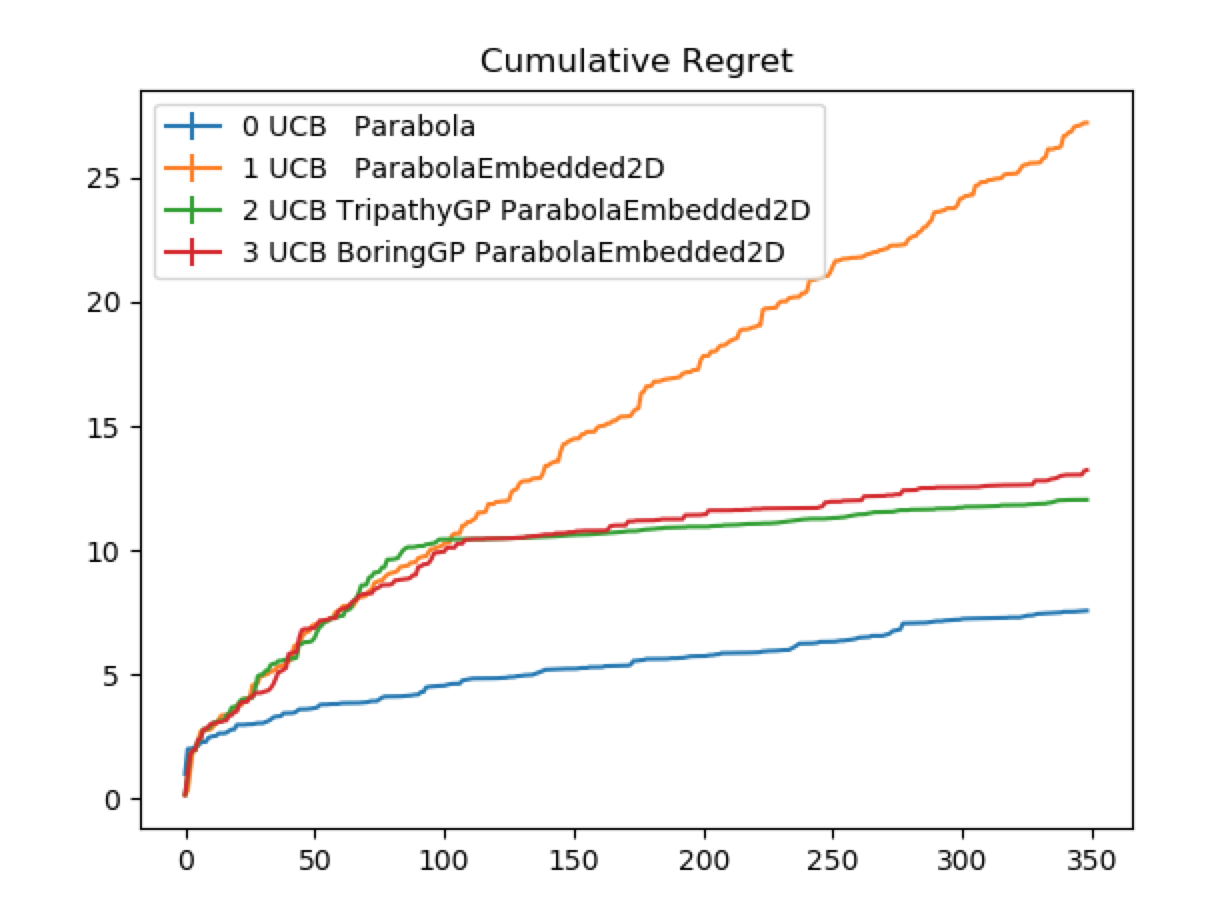
\includegraphics[width=0.5\textwidth]{reference_W_true/Parabola2D}
  \caption{UCB on a Parabola embedded in 2D space, when we assume that tripathy's method finds the real projection matrix.}
\end{figure}

\paragraph{Assume $\hat{W} \neq W_{\text{true}}$}: I now proceed with how different algorithms perform on the function described above.
This measures how the algorithm performs, when subspace identification is a part of the optimization process.

\begin{figure}[H]
  \centering
      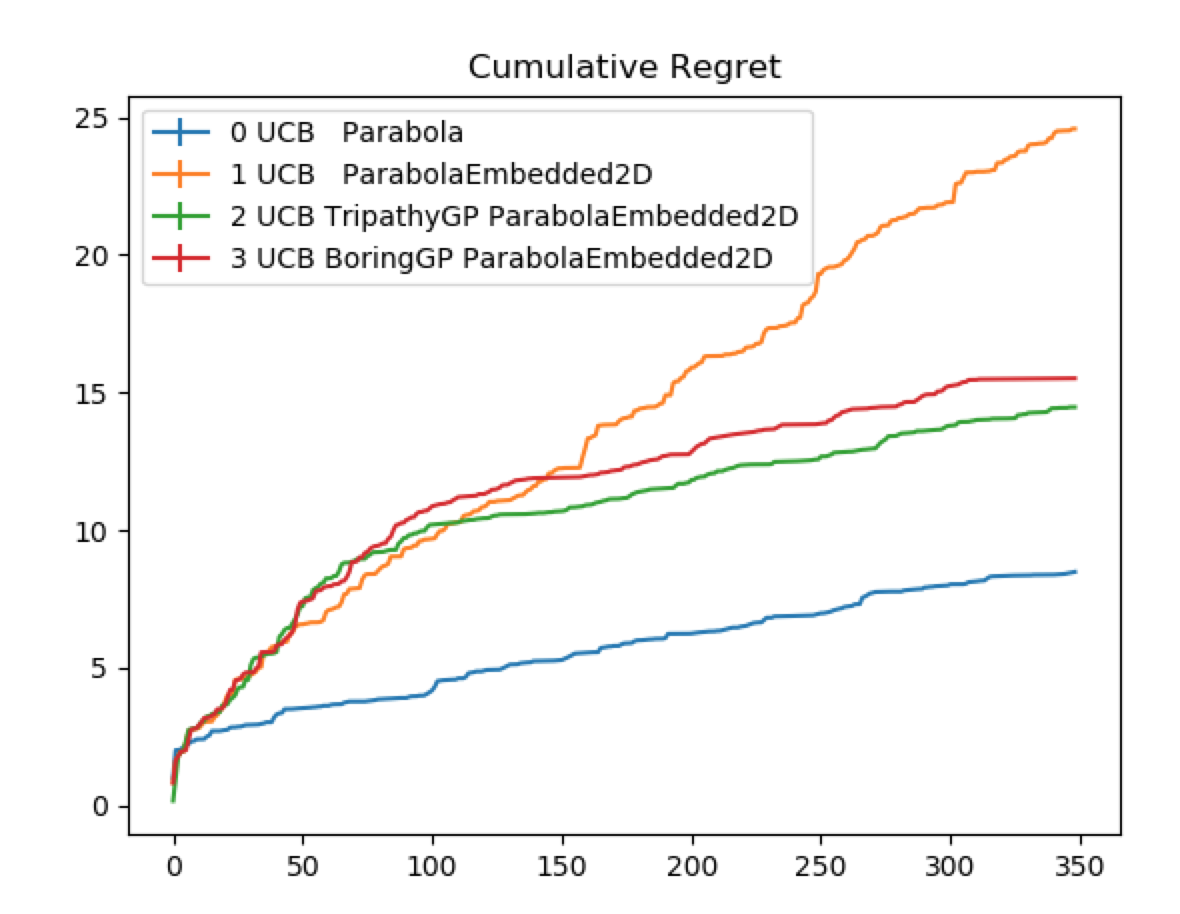
\includegraphics[width=0.5\textwidth]{W_hat_tripathy/Parabola2D_0}
  \caption{UCB on a Parabola embedded in 2D space.
  Tripathy's algorithm is applied to find the a projection matrix $\hat{W}$.}
\end{figure}

One can easily see that the performance on UCB using tripathy's matrix identification algorithm is similar to the case, when we assume that tripathy executes perfectly.


%One can see that REMBO without interleavings has very high variance amongst runs. 
%Sometimes it is able to find a suitable subspace (subfigure (c) and (d)), but on other runs, it fails to find an appropriate subspace.
%The reader should notice that most of these lines are linear.
%This may be the result of not tuning the hyperparameters during runs.
%In this case, the BORING algorithm assesses the exact same properties as the tripathy model (as the number of passive dimensions is set to 0), with which the two models perform very similar on the regret curves. \\

\textbf{The log likelihood of the GP w.r.t the collected datapoints} of the tripathy GP with the real matrix is comparable to the log-likelihood of the GP of the tripathy model, where the active projection matrix is calculated using the algorithm (values of $-1.37$ and $-1.38$ or for a different run values of $195.32$ and $210.25$, where ranges are between  $-100$ and $700$).
One should notice, however, that the angle between the found matrix and the real projection matrix is almost always at $45°$ - a value that does not sound very intuitive, and for which the only reasonable explanation is that the optimization problem stays the same at this projection angle.
The reader can view graphs in a subsequent subsection.

\subsection{Camelback embedded in 3D}

The function to be learned and optimized over is the following:

\def\WCamelback3D{
\begin{bmatrix}
    -0.46554187 & -0.36224966 & 0.80749362 \\
     0.69737806 & -0.711918 & 0.08268378
\end{bmatrix}}

\begin{equation}
f(z_1, z_2) = \left( 4 - 2.1 * z_1^2 + \frac{z_1^4}{3} \right)  z_1^2 + z_1 *  z_2 + \left(-4 + 4 * z_2^2 \right) * z_2^2
\end{equation} \\

where we have $z = \left( \WCamelback3D^T x \right) $, and $ x \in \mathbf{R}^3$, $W \in \mathbf{R}^{2 \times 3}$ and where $z_1$ denotes the first entry of the $z$ vector, and $z_2$ denotes the second element of the $z$ vector.

\paragraph{Assume $\hat{W} = W_{\text{true}}$}: Again, I present how the respective algorithms perform if we assume that Tripathy's Stiefel Manifold optimization finds the perfect matrix.

\begin{figure}[H]
  \centering
      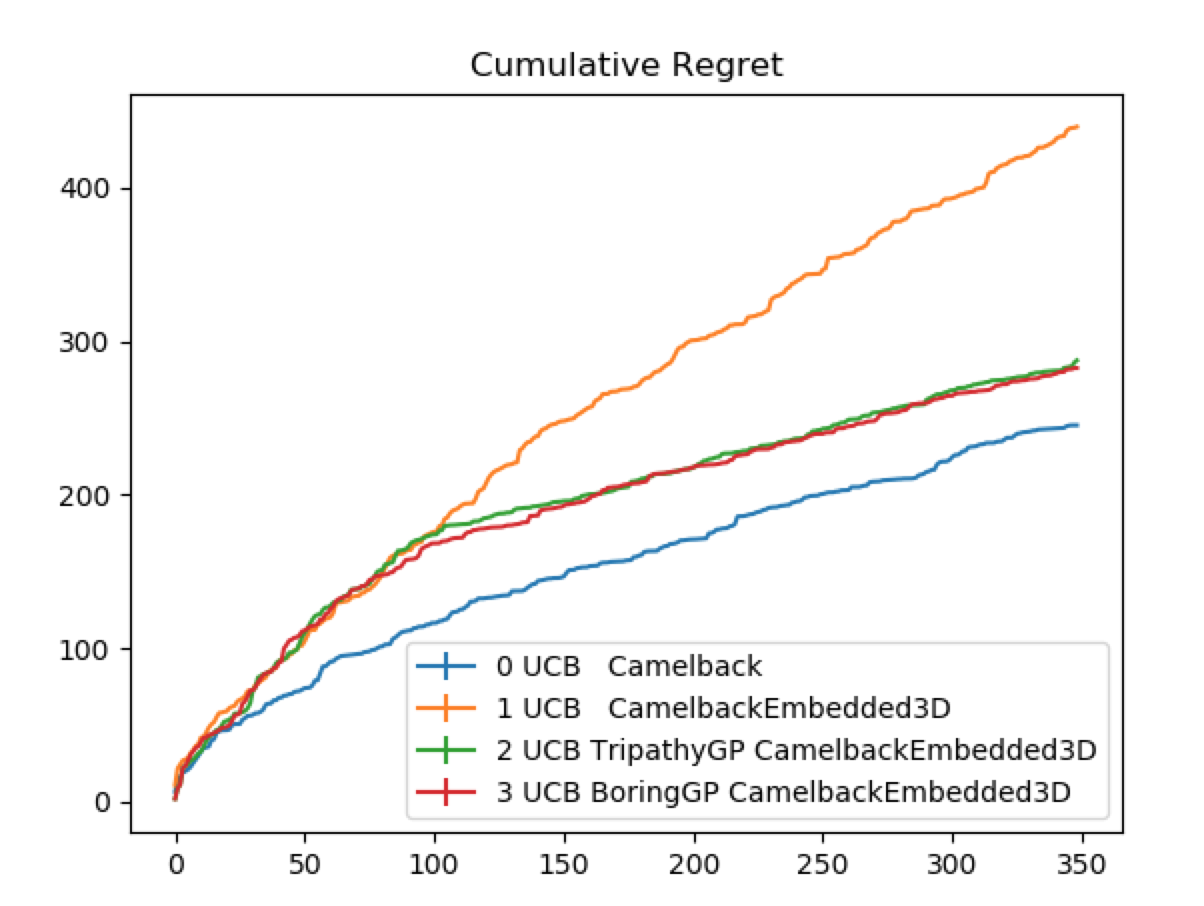
\includegraphics[width=0.5\textwidth]{reference_W_true/Camelback3D}
  \caption{UCB on a 2D Camelback function embedded in 3D space.
  This is when we assume that tripathy finds the real projection matrix $W_{\text{true}}$}
\end{figure}

\paragraph{Assume $\hat{W} \neq W_{\text{true}}$}: Again, I now proceed with the performance, when the subspace identification is part of the optimization process.

\begin{figure}[H]
    \centering
    \begin{subfigure}[b]{0.40\textwidth}
        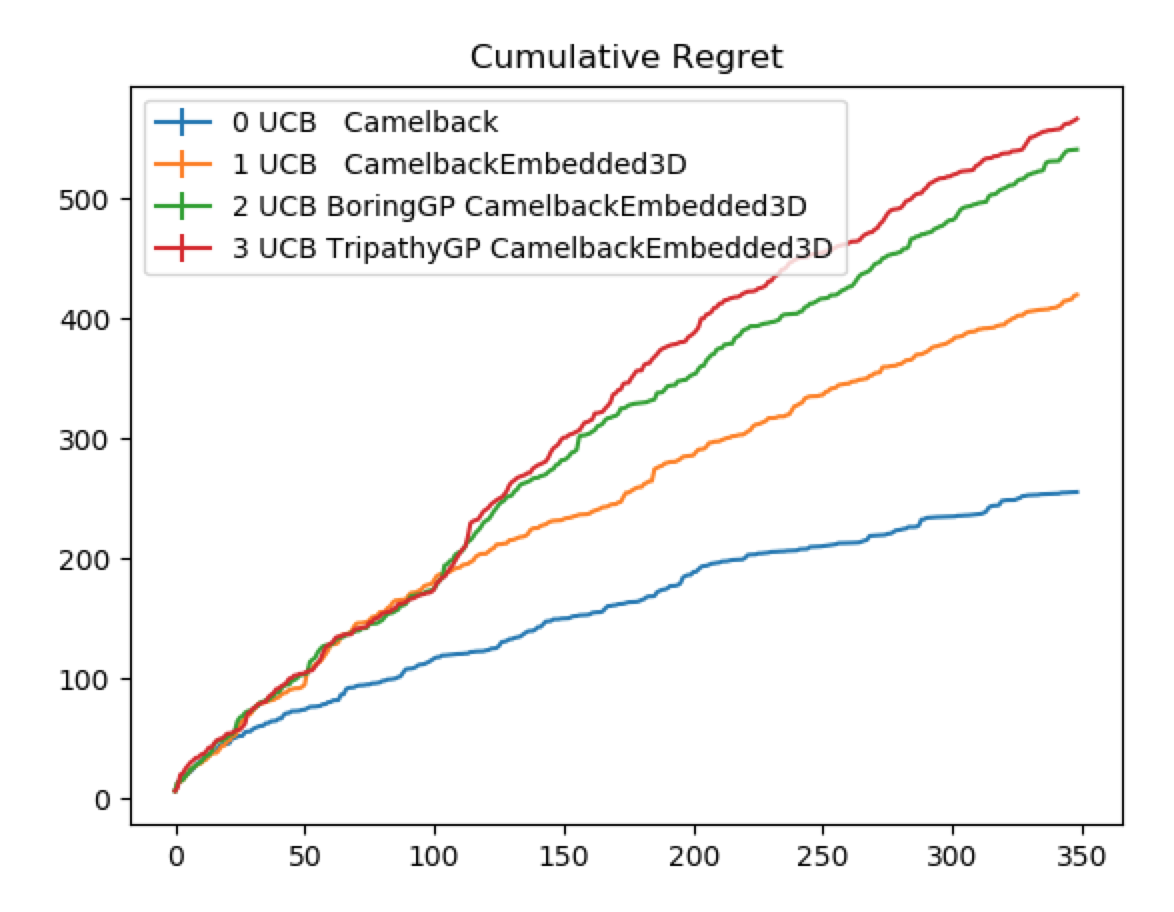
\includegraphics[width=\textwidth]{W_hat_tripathy/Camelback3D_0}
        \label{fig:gull}
    \end{subfigure}
    %add desired spacing between images, e. g. ~, \quad, \qquad, \hfill etc. 
      %(or a blank line to force the subfigure onto a new line)
    \begin{subfigure}[b]{0.40\textwidth}
        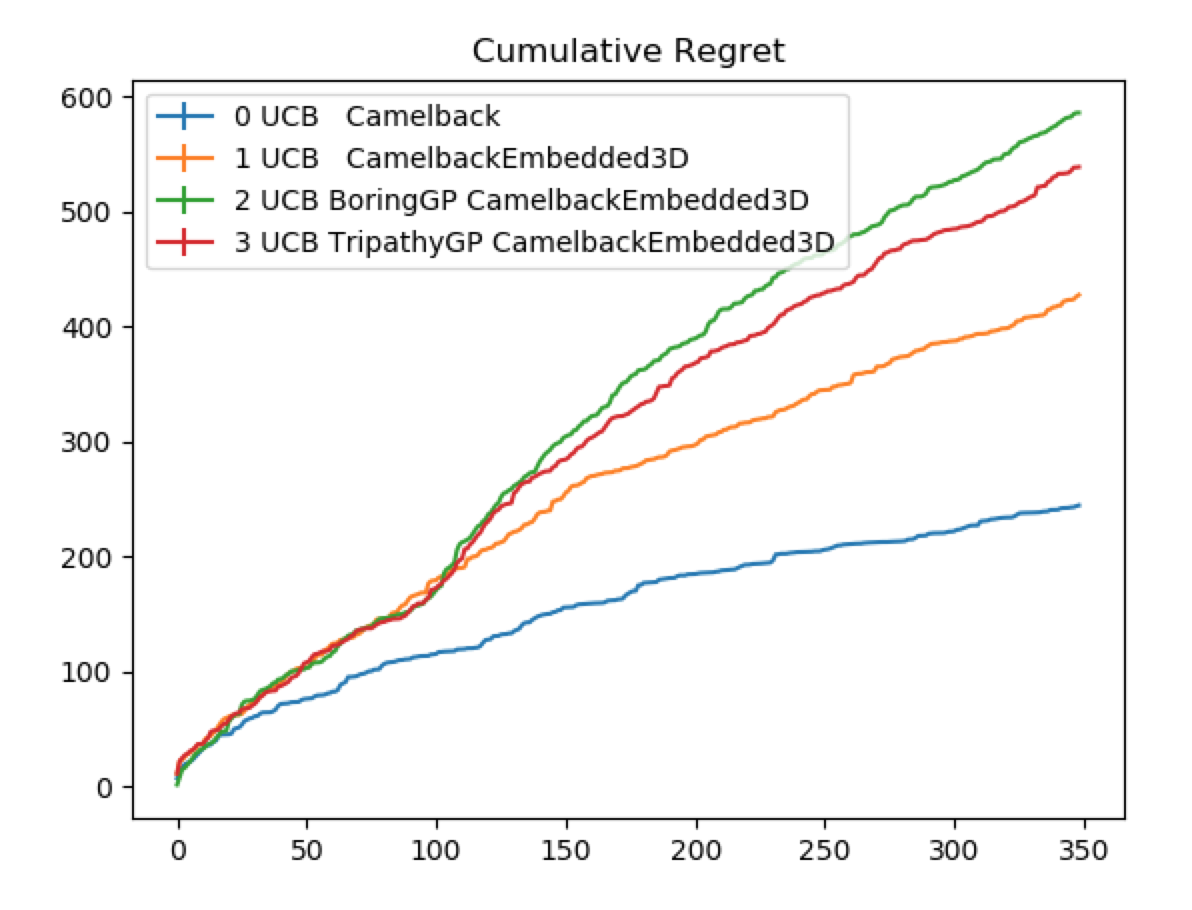
\includegraphics[width=\textwidth]{W_hat_tripathy/Camelback3D_1}
        \label{fig:tiger}
    \end{subfigure}   
        \caption{UCB on a 2D Camelback function embedded in 3D space.
  		We apply tripathy's algorithm to find a projection matrix $W$.}
\end{figure}

One can see that the subspace projection of tripathy's method from 3D to 2D is not efficient. 
The difference between BORING and Tripathy is marginal, as they both rely on a similar algorithm.
This is an indication that the subspace projection is not close to the real subspace, but potentially just finds a subspace which is acceptable when higher dimensions are taken into consideration.
To investigate this further, we increase the dimensionality of the domain in the next section.

\subsection{Camelback embedded in 5D}

\def\WCamelback5D{
\begin{bmatrix}
     -0.31894555 & 0.78400512 & 0.38970008 & 0.06119476 & 0.35776912 \\,
     -0.27150973 & 0.066002 & 0.42761931 & -0.32079484 &-0.79759551
\end{bmatrix}}

\begin{equation}
f(z_1, z_2) = \left( 4 - 2.1 * z_1^2 + \frac{z_1^4}{3} \right)  z_1^2 + z_1 *  z_2 + \left(-4 + 4 * z_2^2 \right) * z_2^2
\end{equation} \\

where we have \\
$z = \left( \WCamelback5D^T x \right) $, and $ x \in \mathbf{R}^5$, $W \in \mathbf{R}^{2 \times 5}$
and where $z_1$ denotes the first entry of the $z$ vector, and $z_2$ denotes the second element of the $z$ vector.

\paragraph{Assume $\hat{W} = W_{\text{true}}$}: The following shows how tripathy performs when we assume perfect projection-matrix identification.

\begin{figure}[H]
  \centering
      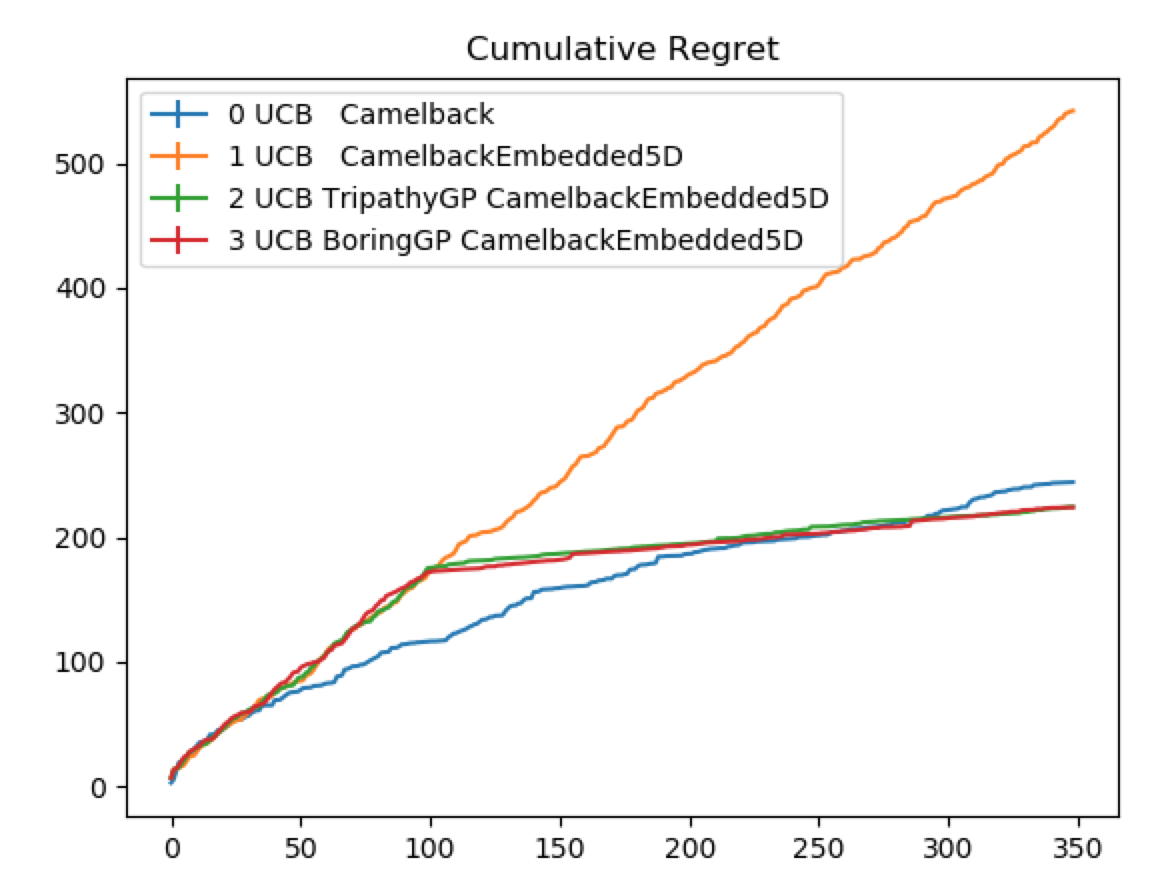
\includegraphics[width=0.5\textwidth]{reference_W_true/Camelback5D}
  \caption{UCB on a 2D Camelback function embedded in 5D space.
  This is when we assume that tripathy finds the real projection matrix $W_{\text{true}}$}
\end{figure}

The linear curve may be the result of kernel parameters that were not set very well, which may lead to the same point chosen repeatedly over and over again.
However, because these kernel parameters are chosen by the algorithm, I do not modify these to get square-root behaved UCB curves.

\paragraph{Assume $\hat{W} \neq W_{\text{true}}$}: The following curves present the performance of UCB when subspace identification is part of the optimization process.

\begin{figure}[H]
    \centering
    \begin{subfigure}[b]{0.40\textwidth}
        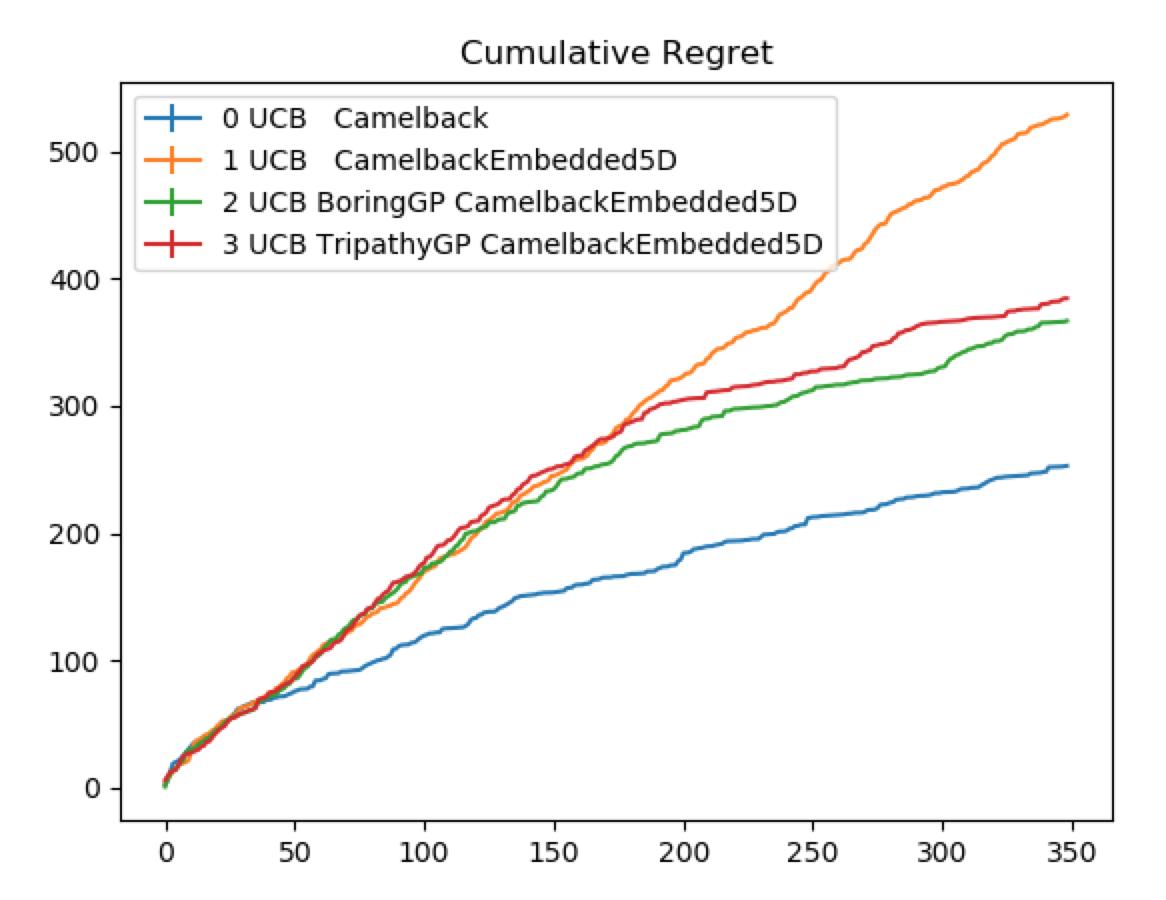
\includegraphics[width=\textwidth]{W_hat_tripathy/Camelback5D_0}
        \label{fig:gull}
    \end{subfigure}
    %add desired spacing between images, e. g. ~, \quad, \qquad, \hfill etc. 
      %(or a blank line to force the subfigure onto a new line)
    \begin{subfigure}[b]{0.40\textwidth}
        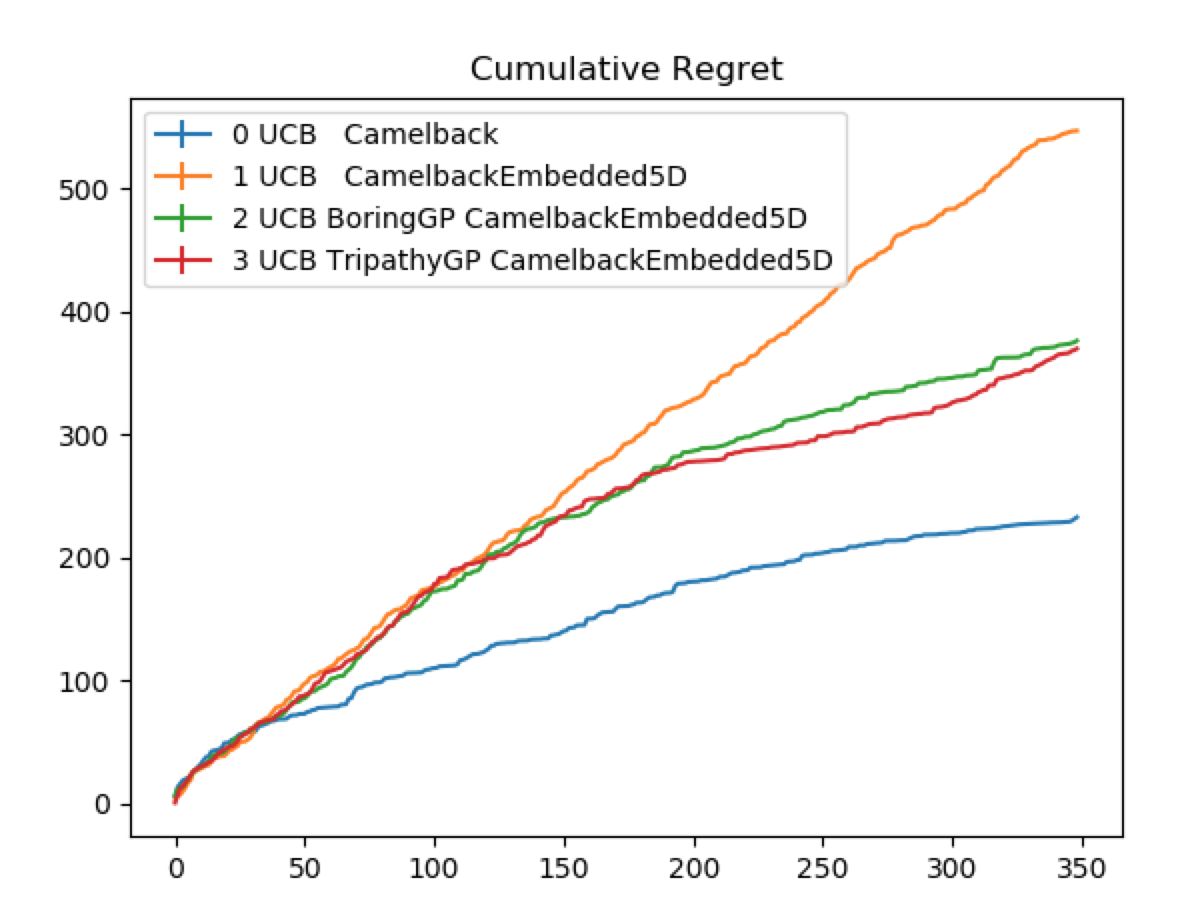
\includegraphics[width=\textwidth]{W_hat_tripathy/Camelback5D_1}
        \label{fig:tiger}
    \end{subfigure}   
           \caption{UCB on a 2D Camelback function embedded in 5D space.
  This is when we apply tripathy's algorithm to find a projection matrix $W$, that is acceptable for optimization, but is not near close to the real projection matrix.}
\end{figure}

One can see for for higher dimensions, tripathy's method performs well, as it is able to reduce the dimensionality of the optimization problem.
However, one can see that the regret achieved from the empirical projection-matrix identification (the real projection-matrix is not found) is much higher.
This poses the question of how well the found projection matrix is compared to the real projection matrix.
I analyse the log-likelihood of the GP to get a quick answer. \\

\textbf{The log likelihood of the GP w.r.t the collected datapoints} of the tripathy GP with the real matrix is not comparable to the log-likelihood of the GP of the tripathy model, where the active projection matrix is calculated using the algorithm.
For different runs, the log-likelihood of the GP including the real matrix is at $-2$ and $-389$, whereas the log-likelihood of the GP with the estimated projection matrix is at $-0.92$ and $-102$. 
Although the values $-2$ and $-0.92$ are close to each other, the pair ($-389$, $-102$) shows that the subspace identification task for this algorithm is much more unstable than that for the parabola.
In the following subsection, I will investigate this issue further.

\subsection{Log-Likelihood and Angle difference measures}

An interesting quantity to take into consideration is the log-likelihood of the sampled data with respect to the GP, and the angle between the found projection matrix, and the real projection matrix.
In the following, I describe how these quantities change over a function of time.
More specifically, the time refers to the number of steps that I allow for tripathy's method to optimize over these parameters.

\paragraph{Parabola}

From the graphs, we can see that the parabola always seems to converge at a projection that is at a 45° to the real projection matrix. 
Intuitively, this seems odd.
One should notice, that the maximum of the optimization problem is the same, when the space is rotated by 45°.
Another explanation could be that 100 datapoints on a 2D space are numerous enough, such that any matrix (that does not directly map to the nullspace of the real projection matrix), is an acceptable matrix).
Why the algorithm always converges at a matrix at 45° to the real projection matrix, would be unclear however in this case.

\begin{figure}[H]
    \centering
    \begin{subfigure}[b]{0.4\textwidth}
        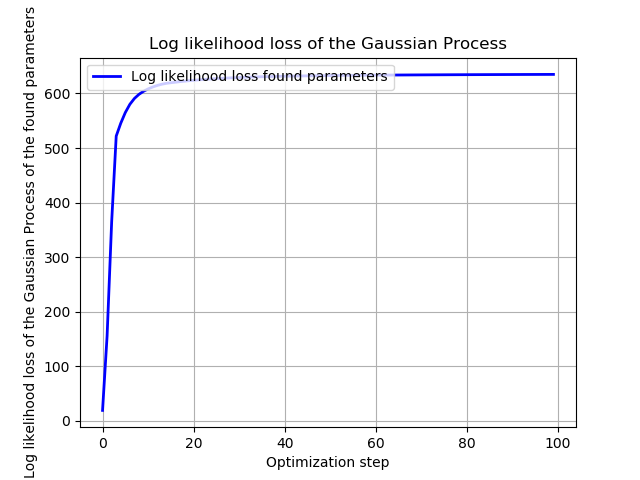
\includegraphics[width=\textwidth]{angles_loss/parabola/Parabola-2D-_1D_20_695_max_run__multiple_loss}
        \label{fig:gull}
           \caption{The momentary $W$ from tripathy's algorithm, and it's log-likelihood w.r.t. the sampled data}
    \end{subfigure}
        \begin{subfigure}[b]{0.40\textwidth}
        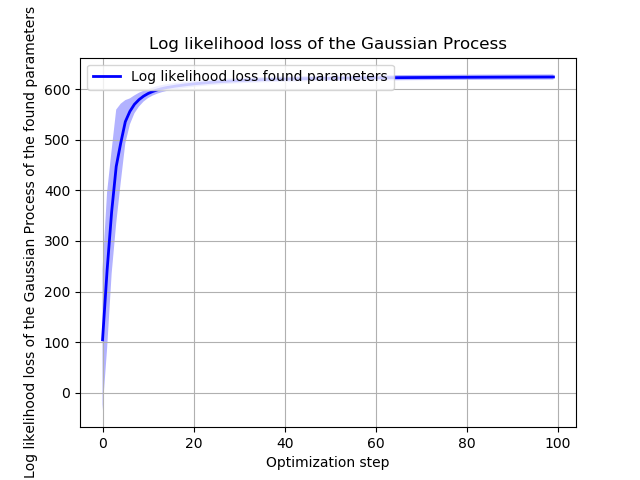
\includegraphics[width=\textwidth]{angles_loss/parabola/Parabola-2D-_1D_20_695_multiple_loss}
        \label{fig:gull}
           \caption{The average of all momentary $W$ from tripathy's algorithm, and it's log-likelihood to the sampled data}
    \end{subfigure}    \vskip\baselineskip
        \begin{subfigure}[b]{0.40\textwidth}
        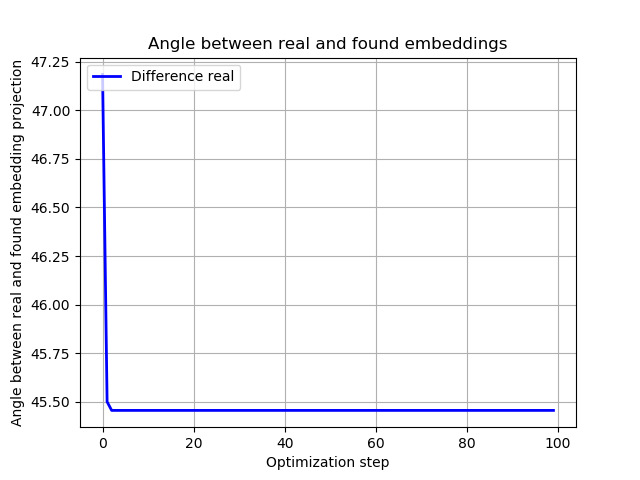
\includegraphics[width=\textwidth]{angles_loss/parabola/Parabola-2D-_1D_20_695_max_run__multiple_angle}
        \label{fig:gull}
           \caption{The momentary $W$ from tripathy's algorithm, and it's angle to the real projection matrix}
    \end{subfigure}
        \begin{subfigure}[b]{0.40\textwidth}
        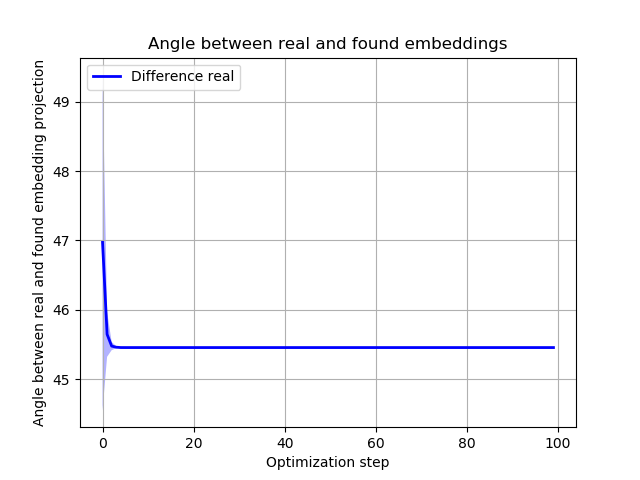
\includegraphics[width=\textwidth]{angles_loss/parabola/Parabola-2D-_1D_20_695_multiple_angle}
        \label{fig:gull}
           \caption{The average of all momentary $W$ from tripathy's algorithm, and it's angle to the real projection matrix}
          \end{subfigure}
    \caption{Log-Likelihood (top) and Angle (bottom) performance measures for a 1D Parabola embedded in a 2D space.
    The left graphs show the values for the run that was chosen as the "found" projection matrix.
    The right graphs show the average values over all restarts of tripathy's method.
    }\label{fig:animals}
\end{figure}

\paragraph{Camelback}
Because from the UCB experiments, we assume Camelback to be more instable, we show the results of two independent runs that exhibit different behavior.
This is evidence, that tripathy's algorithm on Camelback does not run stably, and has high variance (i.e. is not as robust).


\begin{figure}[H]
    \centering
    \begin{subfigure}[b]{0.40\textwidth}
        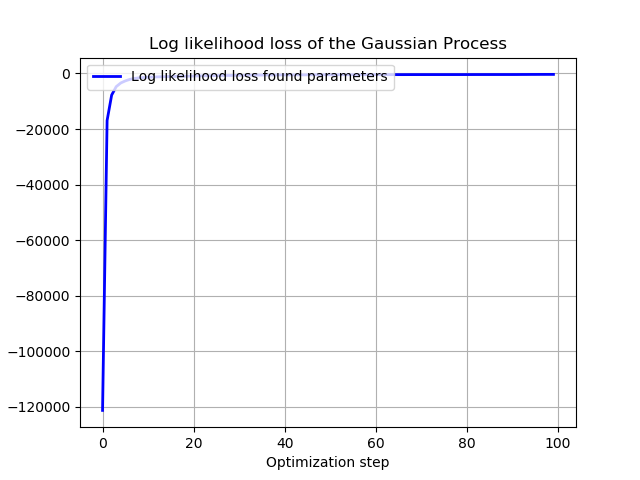
\includegraphics[width=\textwidth]{angles_loss/camelback/run1/Camelback-5D-_2D_20_175_max_run__multiple_loss}
        \label{fig:gull}
                           \caption{The momentary $W$ from tripathy's algorithm, and it's log-likelihood w.r.t the sampled data}
    \end{subfigure}
   \begin{subfigure}[b]{0.40\textwidth}
        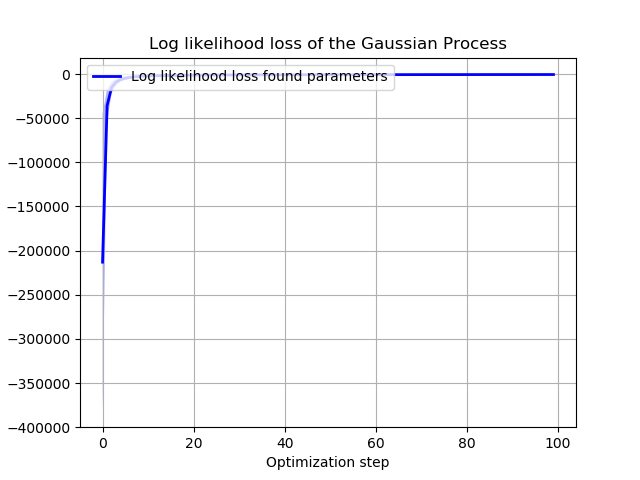
\includegraphics[width=\textwidth]{angles_loss/camelback/run1/Camelback-5D-_2D_20_175_multiple_loss}
        \label{fig:gull}
                           \caption{The average of all momentary $W$ from tripathy's algorithm, and it's log-likelihood w.r.t the sampled data}
    \end{subfigure} 
 \vskip\baselineskip
        \centering
    \begin{subfigure}[b]{0.40\textwidth}
        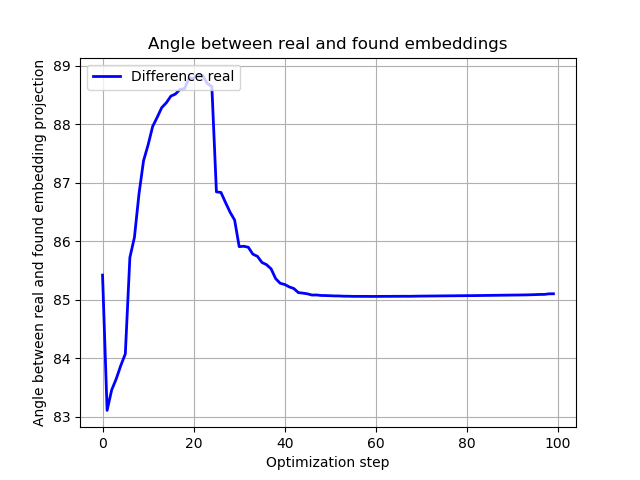
\includegraphics[width=\textwidth]{angles_loss/camelback/run1/Camelback-5D-_2D_20_175_max_run__multiple_angle}
        \label{fig:gull}
               \caption{The momentary $W$ from tripathy's algorithm, and it's angle to the real projection matrix}
    \end{subfigure}
        \begin{subfigure}[b]{0.40\textwidth}
        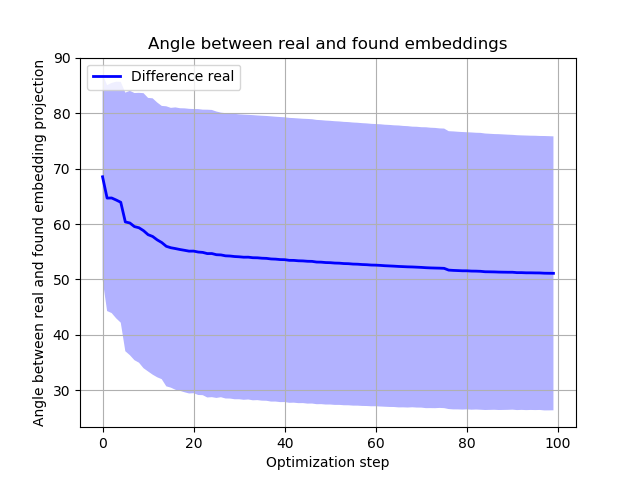
\includegraphics[width=\textwidth]{angles_loss/camelback/run1/Camelback-5D-_2D_20_175_multiple_angle}
        \label{fig:gull}
                           \caption{The average of all momentary $W$ from tripathy's algorithm, and it's angle to the real projection matrix}
    \end{subfigure}
    \caption{Log-Likelihood (top) and Angle (bottom) performance measures for a 2D Camelback  embedded in a 5D space.
    The left graphs show the values for the run that was chosen as the "found" projection matrix.
    The right graphs show the average values over all restarts of tripathy's method.
    These are the results for run 1.
    }\label{fig:animals}
\end{figure}

\begin{figure}[H]
\center
    \begin{subfigure}[b]{0.40\textwidth}
        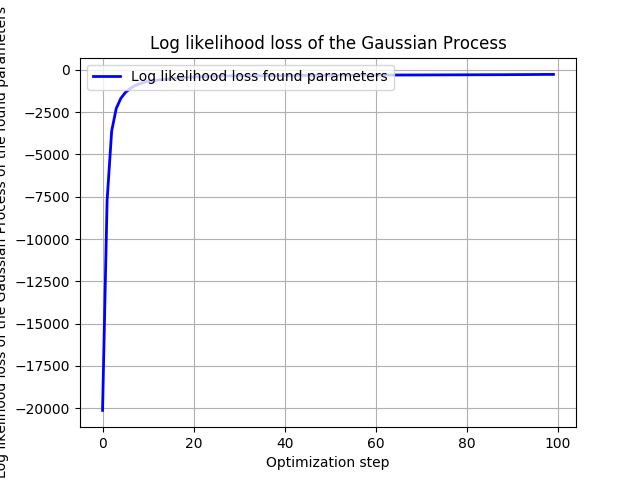
\includegraphics[width=\textwidth]{angles_loss/camelback/run2/Camelback-5D-_2D_20_489_max_run__multiple_loss}
        \label{fig:tiger}                          
         \caption{The momentary $W$ from tripathy's algorithm, and it's log-likelihood w.r.t the sampled data}
    \end{subfigure}   
    \begin{subfigure}[b]{0.40\textwidth}
        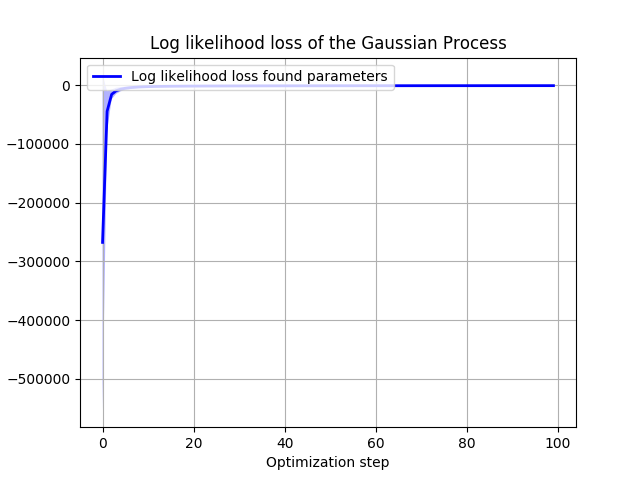
\includegraphics[width=\textwidth]{angles_loss/camelback/run2/Camelback-5D-_2D_20_489_multiple_loss}
        \label{fig:tiger}
               \caption{The momentary $W$ from tripathy's algorithm, and it's angle to the real projection matrix}
    \end{subfigure}   
 \vskip\baselineskip
         \centering
             \begin{subfigure}[b]{0.40\textwidth}
        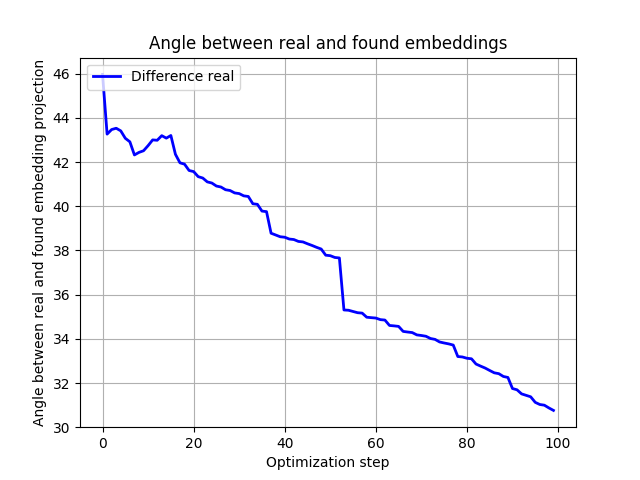
\includegraphics[width=\textwidth]{angles_loss/camelback/run2/Camelback-5D-_2D_20_489_max_run__multiple_angle}
        \label{fig:tiger}                           
        \caption{The average of all momentary $W$ from tripathy's algorithm, and it's log-likelihood w.r.t the sampled data}
    \end{subfigure}
    \begin{subfigure}[b]{0.40\textwidth}
        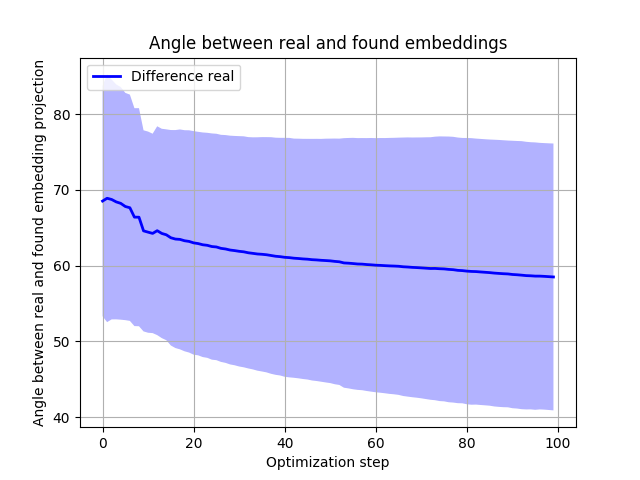
\includegraphics[width=\textwidth]{angles_loss/camelback/run2/Camelback-5D-_2D_20_489_multiple_angle}
        \label{fig:tiger}
               \caption{The average of all momentary $W$ from tripathy's algorithm, and it's angle to the real projection matrix}
    \end{subfigure}   
        \caption{Log-Likelihood (top) and Angle (bottom) performance measures for a 2D Camelback  embedded in a 5D space.
    The left graphs show the values for the run that was chosen as the "found" projection matrix.
    The right graphs show the average values over all restarts of tripathy's method.
    These are the results for run 2.
    }\label{fig:animals}
\end{figure}


\paragraph{Sinusoidal}: 
Although we don't show the UCB curves for the sinusoidal (which also prove to be successful, when this 2d function is hidden within a 5D space), good results can be obtained for subspace identification.

\begin{figure}[H]
\center
    \begin{subfigure}[b]{0.40\textwidth}
        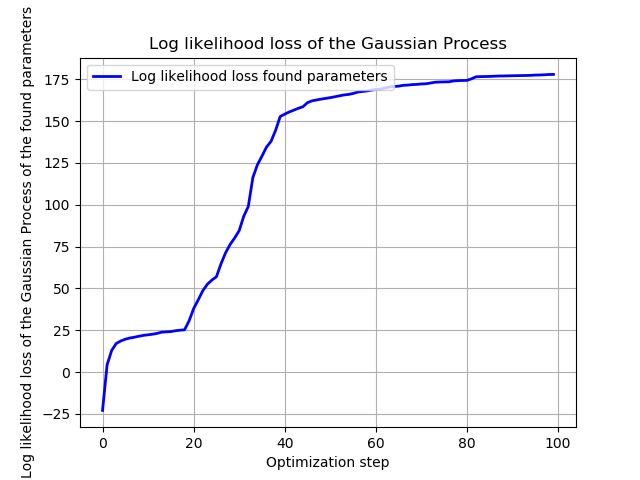
\includegraphics[width=\textwidth]{angles_loss/sinusoidal/Sinusoidal-5D-_2D_20_341_max_run__multiple_loss}
        \label{fig:gull}
         \caption{The momentary $W$ from tripathy's algorithm, and it's log-likelihood w.r.t the sampled data}
    \end{subfigure}
        \begin{subfigure}[b]{0.40\textwidth}
        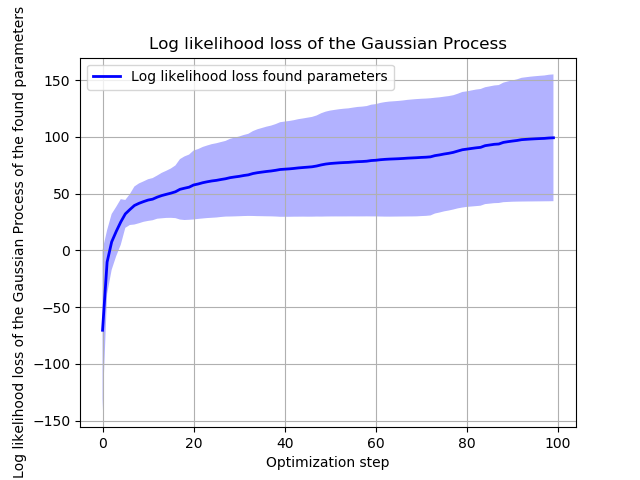
\includegraphics[width=\textwidth]{angles_loss/sinusoidal/Sinusoidal-5D-_2D_20_341_multiple_loss}
        \label{fig:gull}
        \caption{The average of all momentary $W$ from tripathy's algorithm, and it's log-likelihood w.r.t the sampled data}
    \end{subfigure}

 \vskip\baselineskip
         \centering           

    \begin{subfigure}[b]{0.40\textwidth}
        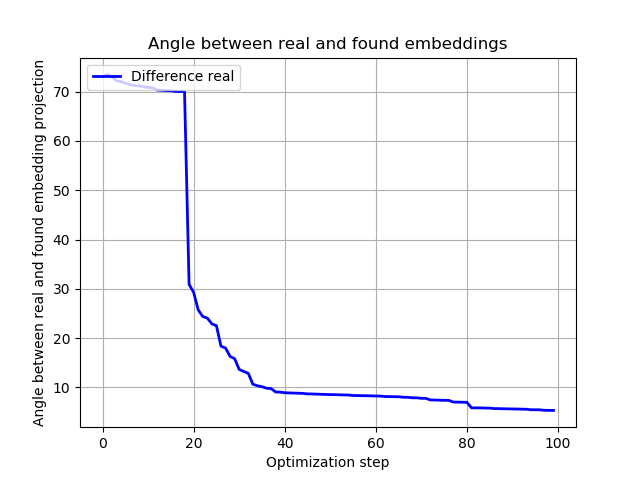
\includegraphics[width=\textwidth]{angles_loss/sinusoidal/Sinusoidal-5D-_2D_20_341_max_run__multiple_angle}
        \label{fig:gull}
               \caption{The momentary $W$ from tripathy's algorithm, and it's angle to the real projection matrix}
    \end{subfigure}
    \begin{subfigure}[b]{0.40\textwidth}
        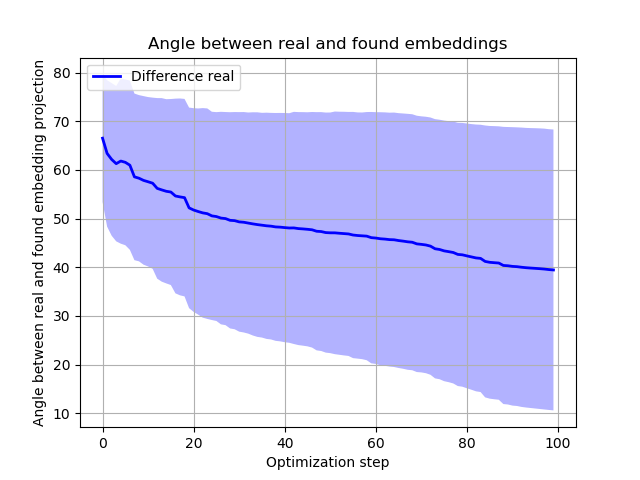
\includegraphics[width=\textwidth]{angles_loss/sinusoidal/Sinusoidal-5D-_2D_20_341_multiple_angle}
        \label{fig:gull}
               \caption{The average of all momentary $W$ from tripathy's algorithm, and it's angle to the real projection matrix}
    \end{subfigure}
           
        \caption{Log-Likelihood (top) and Angle (bottom) performance measures for a 2D Sinusoidal function  embedded in a 5D space.
    The left graphs show the values for the run that was chosen as the "found" projection matrix.
    The right graphs show the average values over all restarts of tripathy's method.
    These are the results for run 2.
    }\label{fig:animals}
\end{figure}

\section{REMBO}

The final algorithm I am investingating is REMBO, as described in chapter 2.
REMBO generally finds good embeddings under the assumption, that optimization domain is normalized, and scaled to $[-\sqrt{d}, \sqrt{d}]^d$ where $d$ is at least the effective dimensionality of the optimization function at hand. \\

I shortly present results for UCB that use REMBO as their optimization algorithm.
The high probability of failing implies a high variance amongst runs. 
As such, I perform 3 runs for each function addressed in the above section.

\paragraph{Parabola}
As one can see, REMBO usually finds an embedding that is acceptable and accelerates the optimization process.
However, run 2 shows that it can also fail in the simplest case of the parabola.
In this regards, tripathy's method is more robust, as it does use some sort of heuristic to check if the chosen matrix delivers good results.


\begin{figure}[H]
\center
    \begin{subfigure}[b]{0.30\textwidth}
        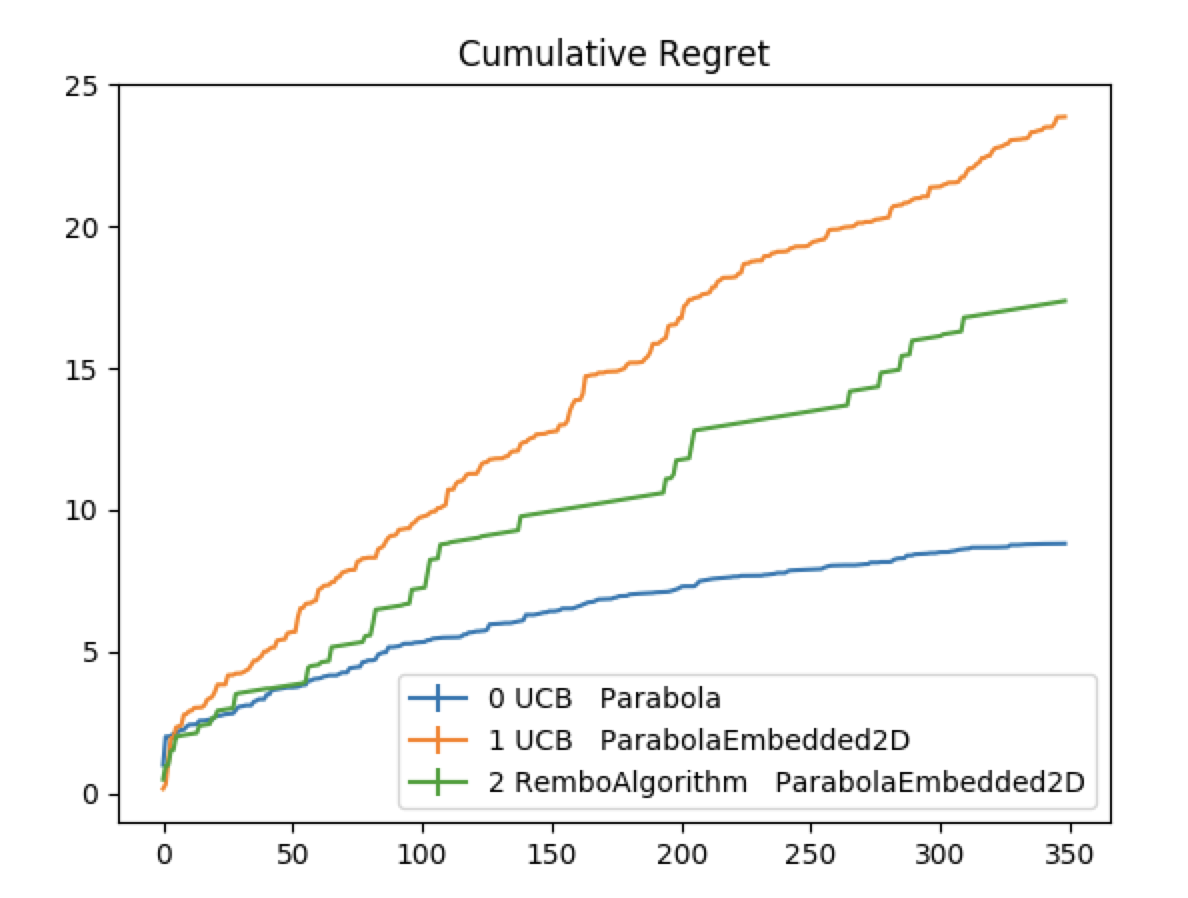
\includegraphics[width=\textwidth]{rembo/Parabola_run0}
        \label{fig:gull}
         \caption{Run 1}
    \end{subfigure}
        \begin{subfigure}[b]{0.30\textwidth}
        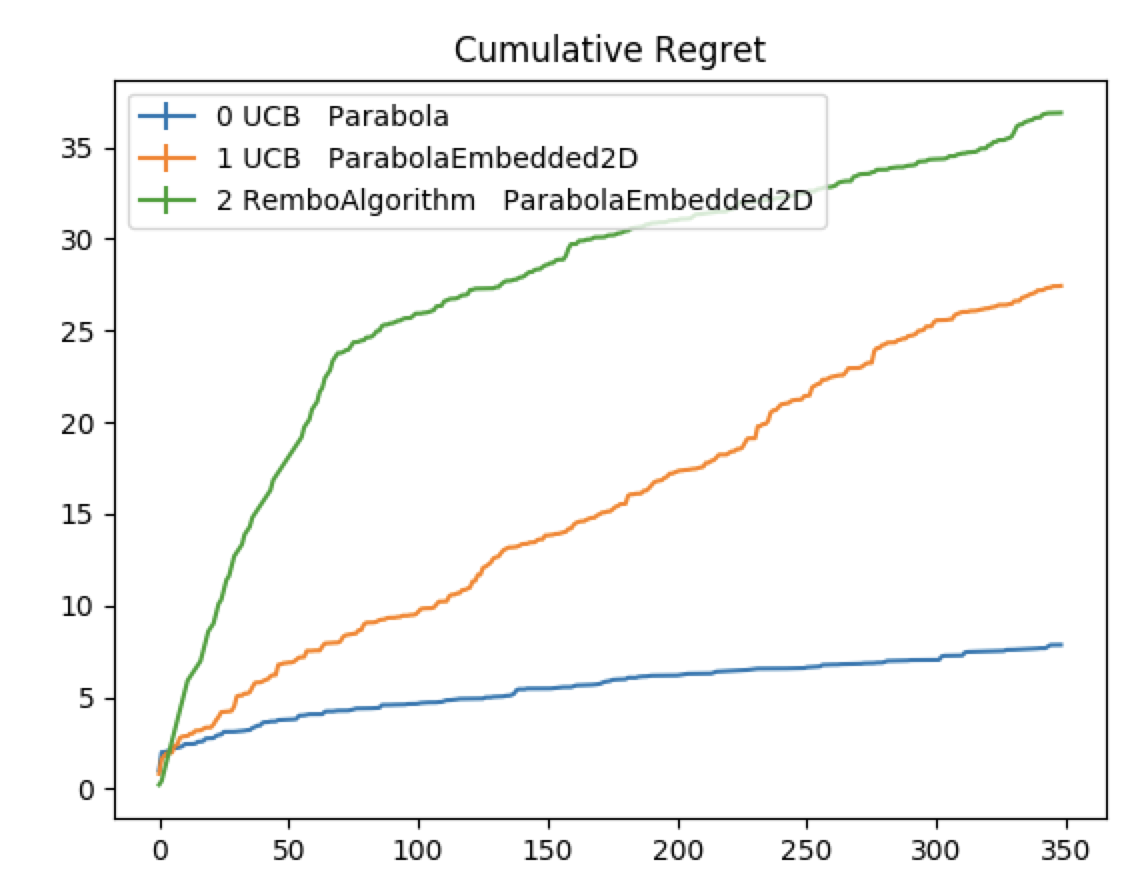
\includegraphics[width=\textwidth]{rembo/Parabola_run1}
        \label{fig:gull}
        \caption{Run 2}
    \end{subfigure}
    \begin{subfigure}[b]{0.30\textwidth}
        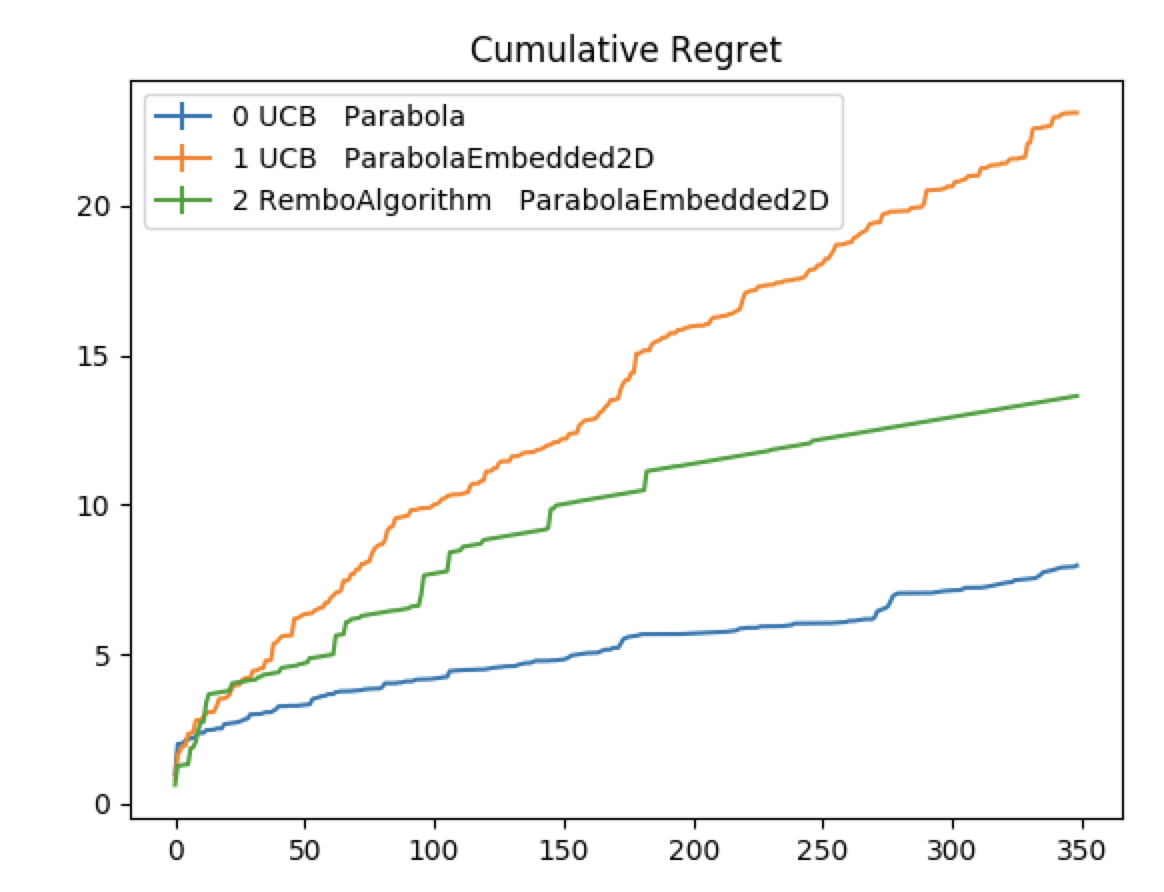
\includegraphics[width=\textwidth]{rembo/Parabola_run2}
        \label{fig:gull}
               \caption{Run 3}
    \end{subfigure}
        \caption{UCB using REMBO on a 1D Parabola embedded in a 2D space.
    }\label{fig:animals}
\end{figure}

\paragraph{Camelback3D}
This example illustrates how REMBO can find an acceptable subspace.
However, the linear lines are an indication for the hyperparameters to be no well chosen. 
I do not allow hyperparameter optimization, for the reason such that the results may be comparable to the other algorithm's results.
As one can see, Camelback3D also provides a difficult for REMBO, although REMBO does find an acceptable subspace projection.

\begin{figure}[H]
\center
    \begin{subfigure}[b]{0.30\textwidth}
        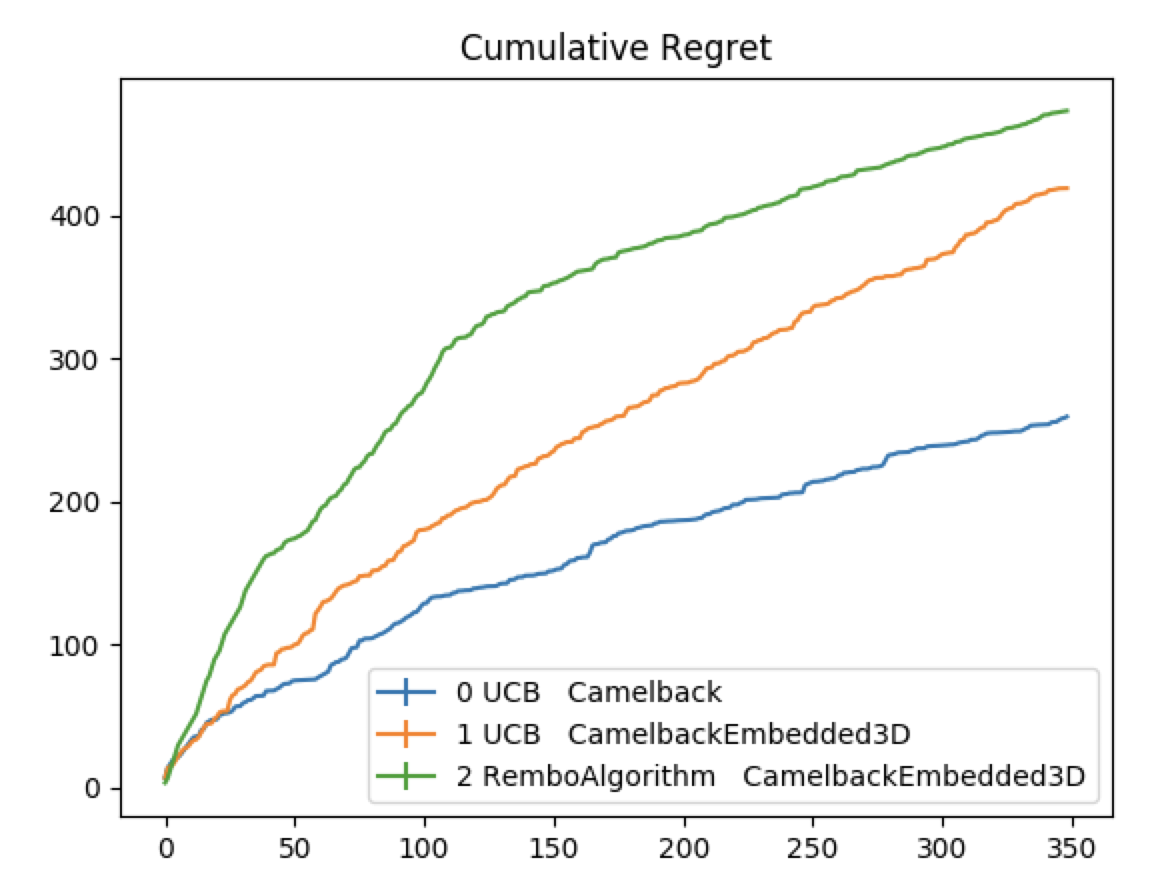
\includegraphics[width=\textwidth]{rembo/Camelback3D_run0}
        \label{fig:gull}
         \caption{Run 1}
    \end{subfigure}
        \begin{subfigure}[b]{0.30\textwidth}
        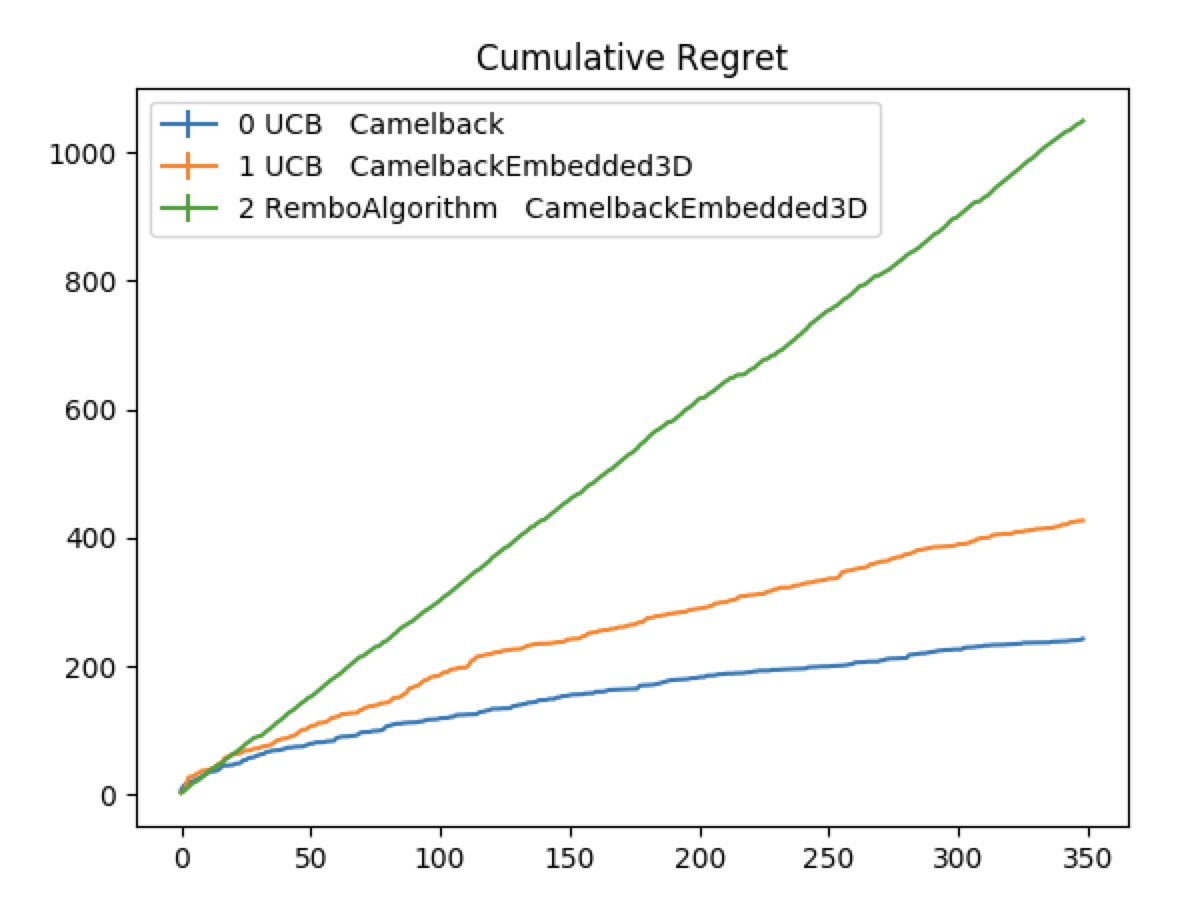
\includegraphics[width=\textwidth]{rembo/Camelback3D_run1}
        \label{fig:gull}
        \caption{Run 2}
    \end{subfigure}
    \begin{subfigure}[b]{0.30\textwidth}
        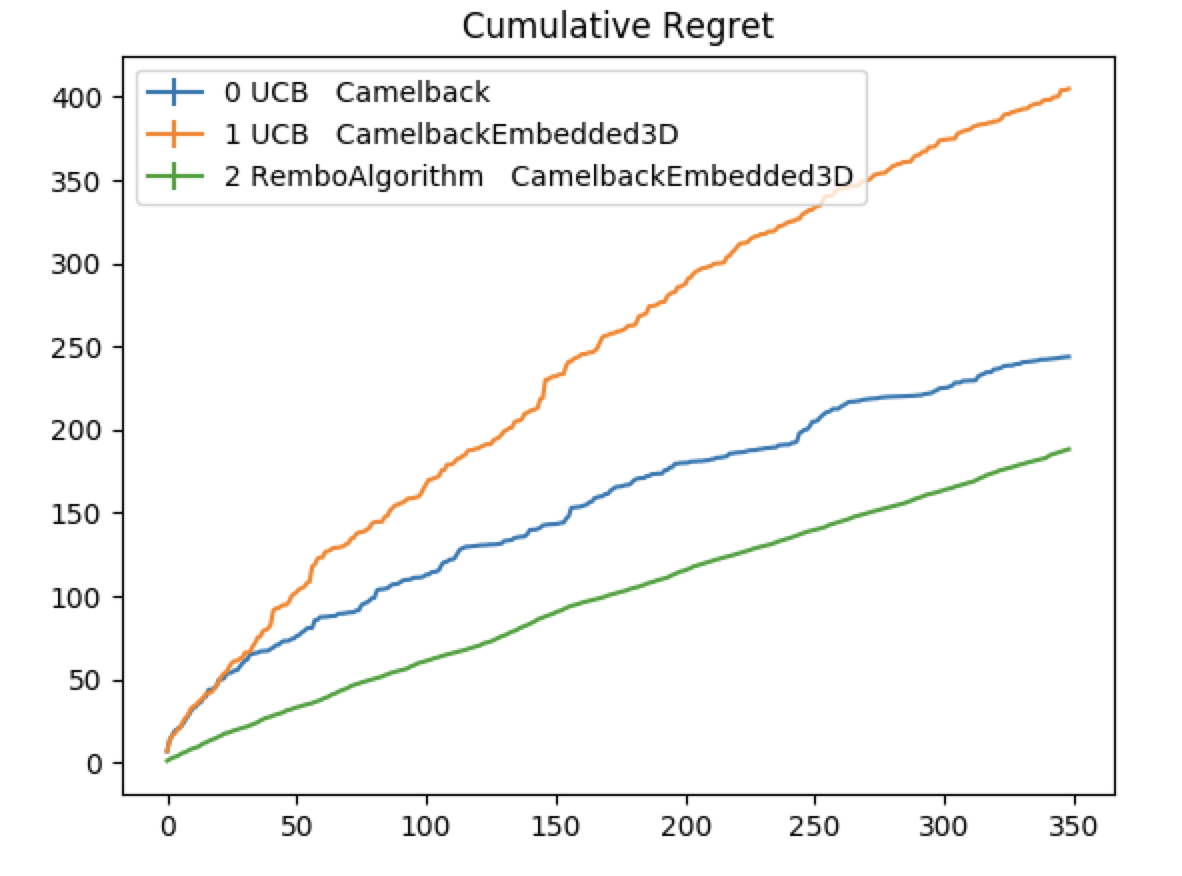
\includegraphics[width=\textwidth]{rembo/Camelback3D_run2}
        \label{fig:gull}
               \caption{Run 3}
    \end{subfigure}
        \caption{UCB using REMBO on a 2D Camelback embedded in a 3D space.
    }\label{fig:animals}
\end{figure}

\paragraph{Camelback5D}
This example illustrates how REMBO can find an acceptable subspace.
However, the linear lines are an indication for the hyperparameters to be no well chosen. 
I do not allow hyperparameter optimization, for the reason such that the results may be comparable to the other algorithm's results.
As one can see, Camelback3D also provides a difficult for REMBO, although REMBO does find an acceptable subspace projection.

\begin{figure}[H]
\center
    \begin{subfigure}[b]{0.30\textwidth}
        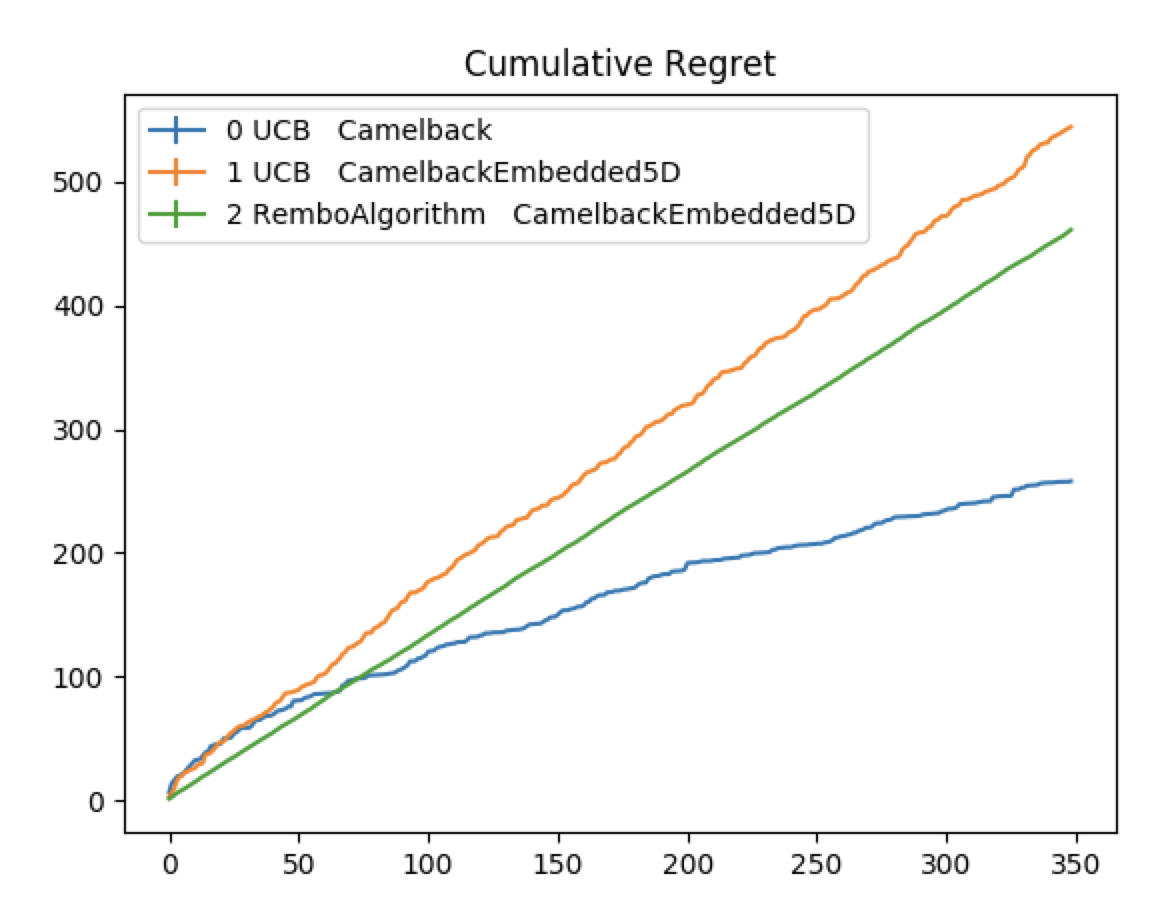
\includegraphics[width=\textwidth]{rembo/Camelback5D_run0}
        \label{fig:gull}
         \caption{Run 1}
    \end{subfigure}
        \begin{subfigure}[b]{0.30\textwidth}
        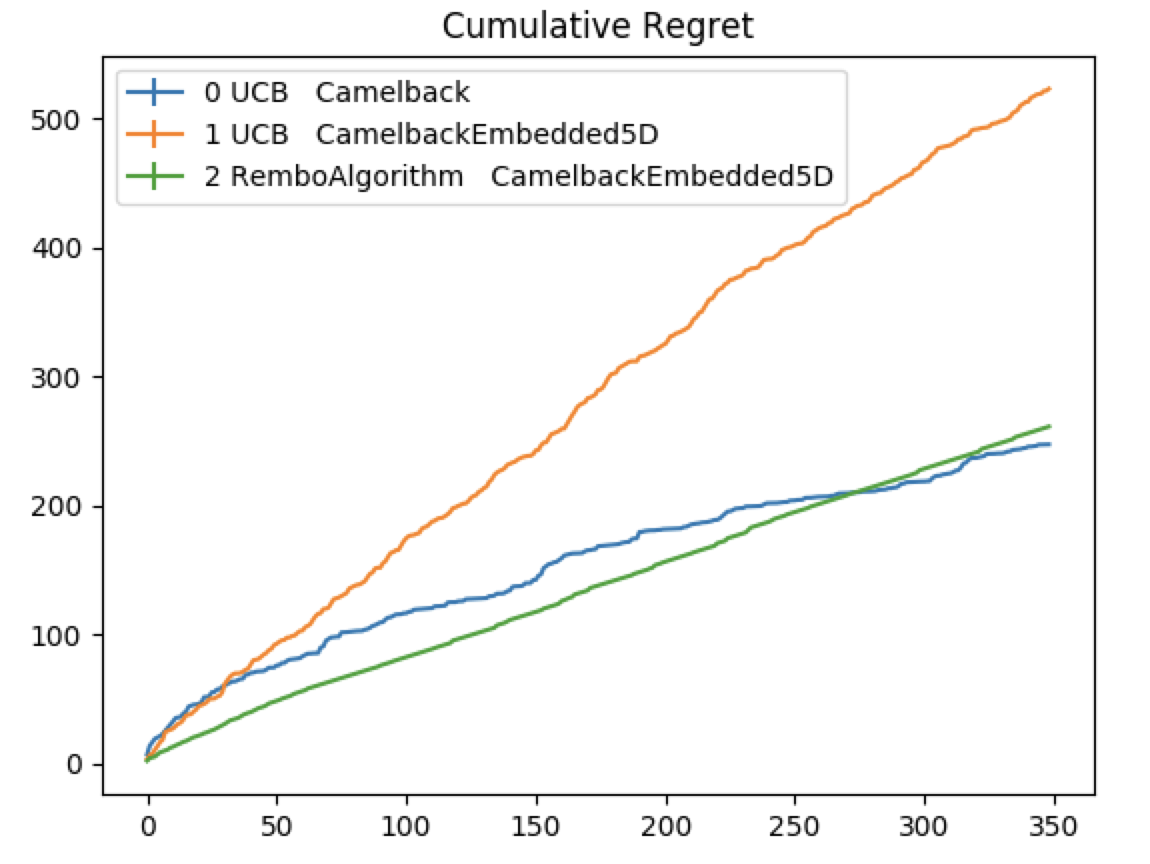
\includegraphics[width=\textwidth]{rembo/Camelback5D_run1}
        \label{fig:gull}
        \caption{Run 2}
    \end{subfigure}
    \begin{subfigure}[b]{0.30\textwidth}
        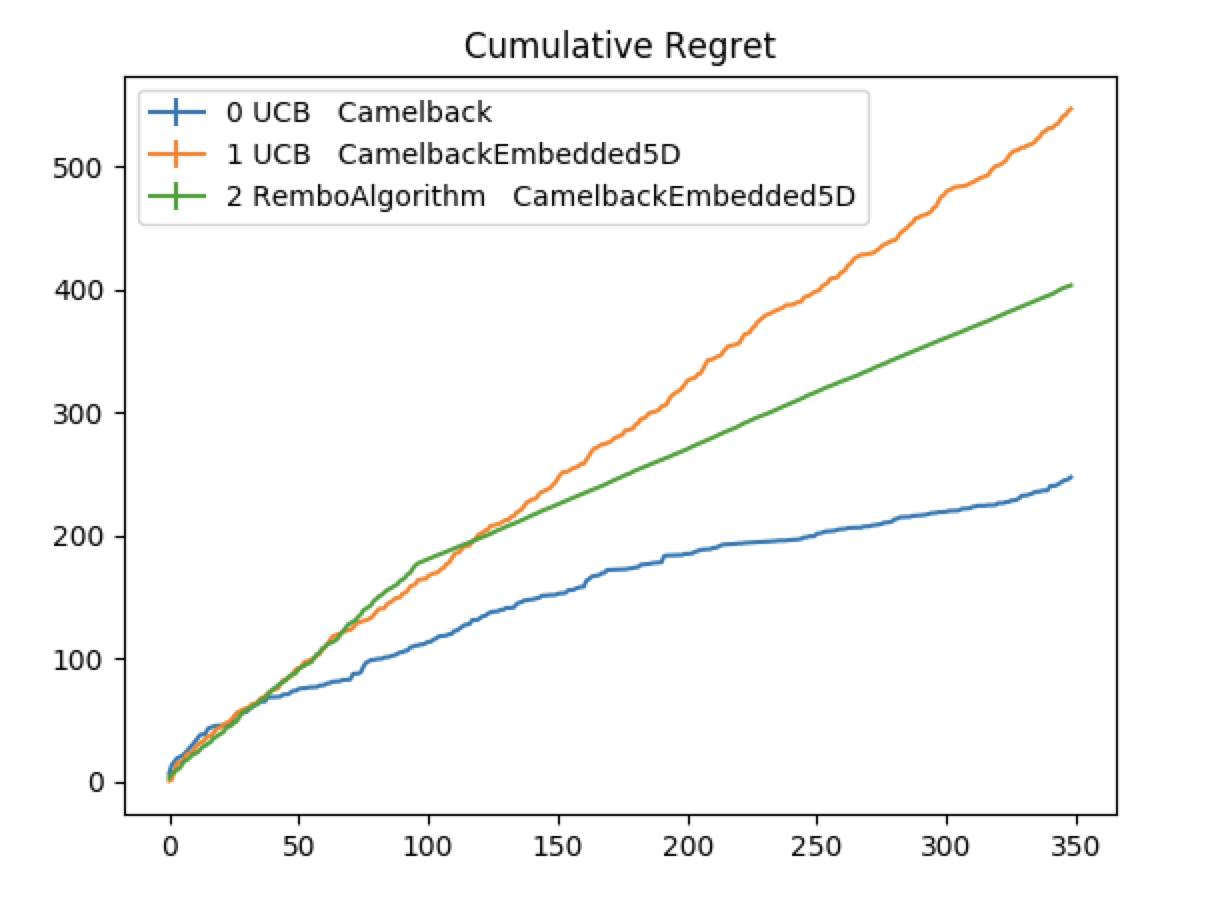
\includegraphics[width=\textwidth]{rembo/Camelback5D_run2}
        \label{fig:gull}
               \caption{Run 3}
    \end{subfigure}
        \caption{UCB using REMBO on a 2D Camelback embedded in a 5D space.
    }\label{fig:animals}
\end{figure}








\begin{enumerate}
\item Show UCB runs for the same runs as the funtions used for tripathy/boring
\item Talk about high variance in results
\item Talk about parameters are very sensitive
\item Talk about choosing the optimization domain
\item Talk about having no measure of knowing if the embedding is good or not.
\end{enumerate}




\section{Qualitative evaluation}
It is interesting to see, that amongst the 1000 restarts that I generated, some of the resulting matrices are close to the real projection matrix up to an absolute value of 0.01.
However, because the algorithm decides to choose the matrix with the highest likelihood, tripathy's algorithm in general does not select these matrices, but chooses a matrix that is not amongst the matrices that are very similar to the real matrices.

\subsection{Feature selection}
The goal of this task is to see, if the revised active subspace identification algorithms can effectively do feature selection.
For this task, I set up a function $ f $ that looks as follows:

\def\B{
\begin{bmatrix}
    (x - a_0)^2 \\
    (y - a_1)^2
\end{bmatrix}}

\begin{equation} \label{eq:FeatureExtension}
f \left( W \B \right) \approx g \left( x \right)
\end{equation} 

where $x_0, x_1$ are constants. \\

For this specific experiment, the function $f$ is chosen to be a one-dimensional parabola. 
As such, $W$ is chosen as a matrix on the Stiefel manifold with dimensions $\mathbf{R}^{d \times D}$

Doing a feature extension over $x$ and $y$, we can get the following feature representation:

\def\PHI{
\begin{bmatrix}
	x_0^2 \\
	x_1^2 \\
	x_0 \\
	x_1 \\
    1
\end{bmatrix}}


\def\WtoPhi{
\begin{bmatrix}
	w_0 \\
    w_1 \\
	-2 w_0 a_0 \\
	-2 w_1 a_1 \\
	w_0 a_0^2 + w_1 a_1^2
\end{bmatrix}}

\begin{figure}[h]

\begin {minipage}{0.47\textwidth}
  \centering
  \begin{equation}
    \PHI
  \end{equation}
  \caption{Polynomial Kernel applied to vector $[x_0, x_1]$}
\end{minipage}
\hfill
\begin {minipage}{0.47\textwidth}
  \centering
  \begin{equation}
    \WtoPhi
  \end{equation}
  \caption{Corresponding weight matrix equivalent to \ref{eq:FeatureExtension} when applied on a parabola}
\end{minipage}

\end{figure}

To run experiments, I instantiate the "real" matrix, which should be found by the algorithm with the values $w_0 = 0.589$, $w_1 = 0.808$ (randomly sampled as a matrix on the Stiefel manifold), $a_0 = -0.1$, $a_1 = 0.1$ (chosen by me as coefficients). \\

I apply the algorithm 1. from \citep{Tripathy} to identify the active projection matrix.
The optimization algorithm has 50 samples to discover the hidden matrix, which it seemingly does up do a certain degree of accuracy.
Similar results are achieved for repeated tries.
The following figure shows the real matrix, and the matrix the algorithm has found.

\def\realW{
\begin{bmatrix}
	0.589 \\
    0.808 \\
	0.118 \\
	-0.162 \\
	0.823
\end{bmatrix}}

\def\okW1{
\begin{bmatrix}
	-0.355 \\
    	-0.533 \\
    	-0.908 \\
    	0.099 \\
    -0.756 
\end{bmatrix}}

\begin{figure}[h] 
\begin {minipage}{0.47\textwidth}
  \centering
  \begin{equation} \label{fig:realMatrix}
    \realW
  \end{equation}
  \caption{Real matrix}
\end{minipage}
\hfill
\begin {minipage}{0.47\textwidth}
  \centering
  \begin{equation} \label{fig:foundMatrix}
    \okW1
  \end{equation}
  \caption{Matrix found by optimization algorithm}
\end{minipage}
\end{figure}

Although one can see that the element wise difference between the two matrices \ref{fig:realMatrix} and \ref{fig:foundMatrix} are high (between $0.05$ and $0.15$), one can see that the matrix recovery is successful in finding an approximate structure that resembles the original structure of the features.
One should observe that the found matrix is an approximate solution to the real matrix in the projection. I.e. the matrix found is close to the real matrix, but multiplied by $-1$. \\

Because in this case, I applied the feature selection algorithm on a vector-matrix (only one column), one can quantify the reconstruction of the real matrix through the found matrix by the normalized scalar product.
This quantity is a metric between $0$ and $1$, where $0$ means that both vectors are orthogonal, and $1$ means that both vectors overlap.

\begin{equation}
\text{overlap}(u, v) = \frac{| \langle u, v \rangle |}{\langle u, u \rangle}
\end{equation}
where $u$ is the real vector, and $v$ is the found vector.

Inserting the actual values into the field, we get $0.79$, which is a good value for the feature vector found, and the trained number of datapoints which is 50. \\
 
 This experiment shows that algorithm 1. from \citep{Tripathy} successfully allows a viable option to other feature selection algorithms, by providing a measure, where the optimal linear projection is found. 
 However, one must notice that other feature selection algorithms (such as SVM), are more efficient, and will provide better results with higher probability if applied on a similar kernel. \\
 
 One major observation I made was the the increase in the log likelihood of the data w.r.t. the projection matrix did not correlate with the decrease in the angle between the real vs the found projection matrix.
 Also, most often, the angle was at around 40 degrees, which means that only slight improvements over a fully random embedding were made.


\subsection{Subspace identification}
One of the main reasons to use our method is because we allow for subspace identification.
We have the following functions:

\begin{enumerate}
\item 1D Parabola embedded in a 2D space
\item 2D Camelback embedded in a 5D space
\item 2D Sinusoidal and Exponential function embedded in a 5D space
\end{enumerate}

To be able to visualize the points, I proceed with the following procedure:

I generate testing points (points to be visualized) within the 2D-space in a uniform grid.
I then project these testing points to the dimension of the original function ($2d$ for parabola, else $5d$).
I then let each algorithm learn and predict the projection matrix and GP mean predictions.
If because the transformation from $2D$ space, to $5D$ space and to GP mean prediction is each bijective, we can visualize the $2D$ points with the GP mean prediction right away.
As such, the dimension of the embedding learned does not have impact on the visualization!

In the following figures, blue point shows the sampled real function value.
Orange points shows the sampled mean prediction of the trained GP.
The GPs were each trained on 100 datapoints. 
The points shown below were not used for training at any point, as these are included in the test-set.

% PARABOLA FUNCTION
\begin{figure}[H]
    \centering
    \begin{subfigure}[b]{0.30\textwidth}
        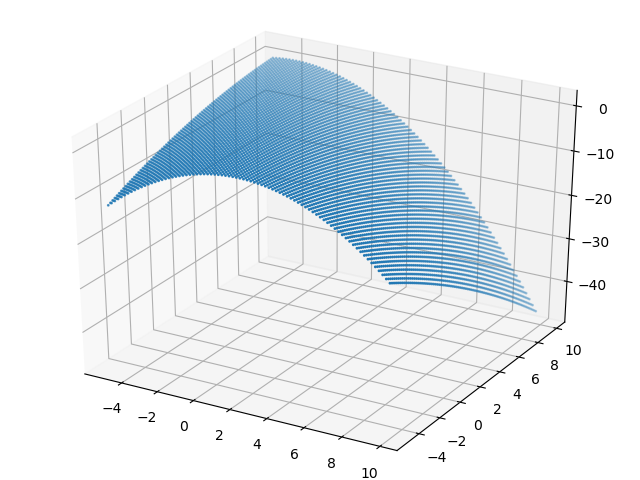
\includegraphics[width=\textwidth]{orig/Parabola-2D-_1D.png}
        \caption{Parabola Original}
        \label{fig:gull}
    \end{subfigure}
    %add desired spacing between images, e. g. ~, \quad, \qquad, \hfill etc. 
      %(or a blank line to force the subfigure onto a new line)
    \begin{subfigure}[b]{0.30\textwidth}
        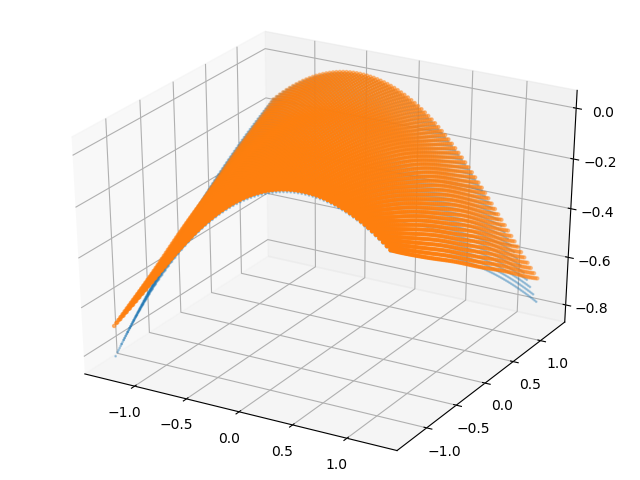
\includegraphics[width=\textwidth]{orig/Parabola-2D-_1D_BORING.png}
        \caption{Parabolanusoidal Boring}
        \label{fig:tiger}
    \end{subfigure}
     %add desired spacing between images, e. g. ~, \quad, \qquad, \hfill etc. 
    %(or a blank line to force the subfigure onto a new line)
    \vskip\baselineskip
    \begin{subfigure}[b]{0.30\textwidth}
        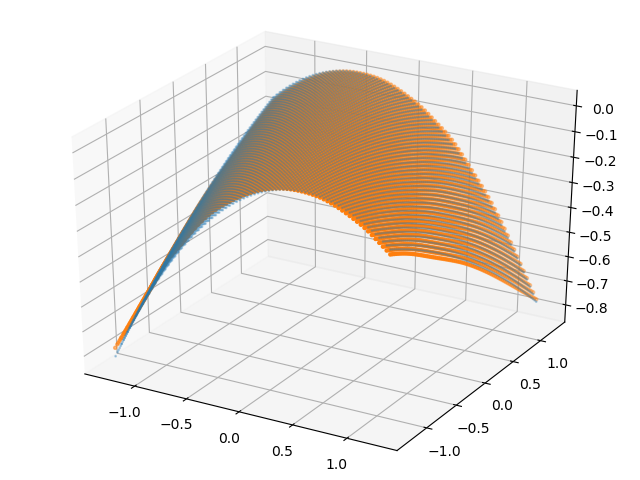
\includegraphics[width=\textwidth]{orig/Parabola-2D-_1D_TRIPATHY.png}
        \caption{Parabola Tripathy}
        \label{fig:mouse}
    \end{subfigure}
            %add desired spacing between images, e. g. ~, \quad, \qquad, \hfill etc. 
    %(or a blank line to force the subfigure onto a new line)
    \begin{subfigure}[b]{0.30\textwidth}
        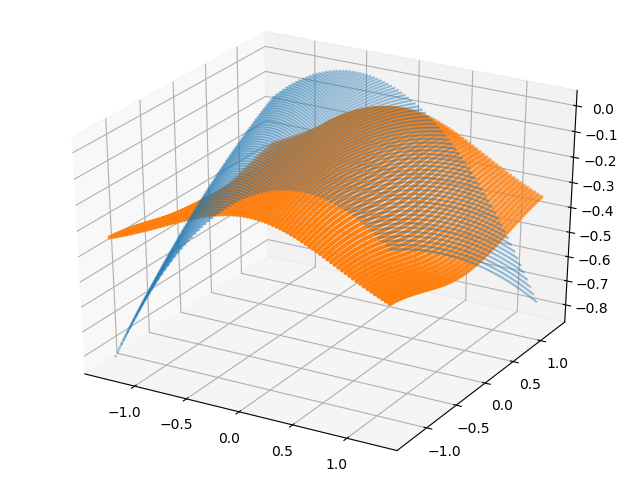
\includegraphics[width=\textwidth]{orig/Parabola-2D-_1D_REMBO.png}
        \caption{Parabola Rembo}
        \label{fig:mouse}
    \end{subfigure}
    \caption{Top-Left: The 1D Parabola which is embedded in a 2D space.}\label{fig:animals}
\end{figure}

I set the number of restarts to $14$ and number of randomly sampled datapoints to 100.
Notice that the Tripathy approximation is slightly more accurate than the BORING approximation. 
This is because one of Tripathy's initial starting points were selected better, such that algorithm 3 ran many times before the relative loss terminated the algorithm.
The active subspace projection matrix is of size $\mathbf{R}^{1 \times 2}$

% SINUSOIDAL FUNCTION
\begin{figure}[H]
    \centering
    \begin{subfigure}[b]{0.3\textwidth}
        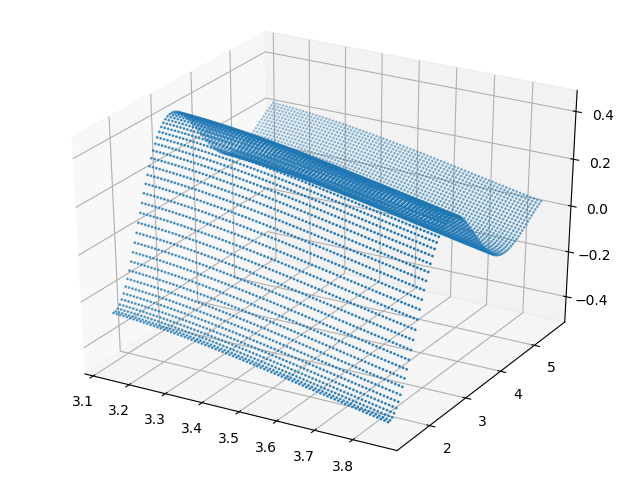
\includegraphics[width=\textwidth]{orig/Sinusoidal-5D-_2D.png}
        \caption{Sinusoidal Original}
        \label{fig:gull}
    \end{subfigure}
    ~ %add desired spacing between images, e. g. ~, \quad, \qquad, \hfill etc. 
      %(or a blank line to force the subfigure onto a new line)
    \begin{subfigure}[b]{0.3\textwidth}
        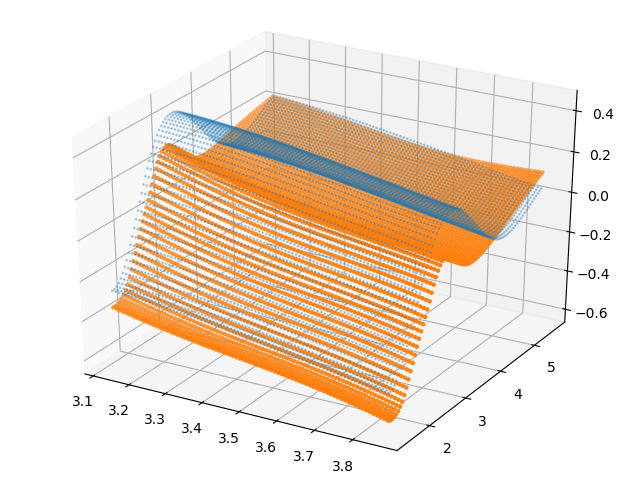
\includegraphics[width=\textwidth]{orig/Sinusoidal-5D-_2D_BORING.png}
        \caption{Sinusoidal Boring}
        \label{fig:tiger}
    \end{subfigure}
        \vskip\baselineskip
 %add desired spacing between images, e. g. ~, \quad, \qquad, \hfill etc. 
    %(or a blank line to force the subfigure onto a new line)
    \begin{subfigure}[b]{0.3\textwidth}
        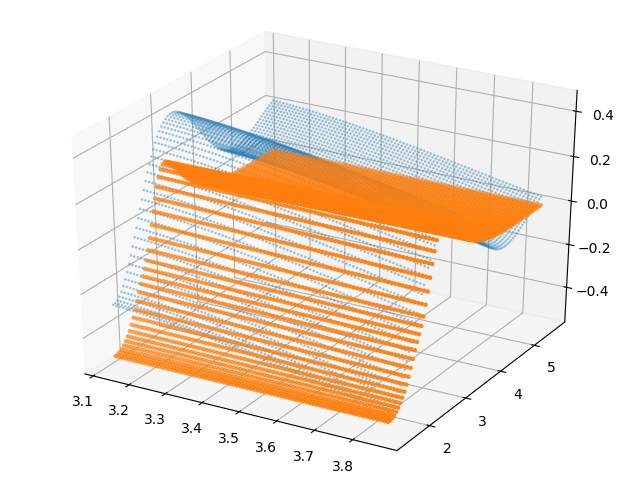
\includegraphics[width=\textwidth]{orig/Sinusoidal-5D-_2D_TRIPATHY.png}
        \caption{Sinusoidal Tripathy}
        \label{fig:mouse}
    \end{subfigure}
        ~ %add desired spacing between images, e. g. ~, \quad, \qquad, \hfill etc. 
    %(or a blank line to force the subfigure onto a new line)
    \begin{subfigure}[b]{0.3\textwidth}
        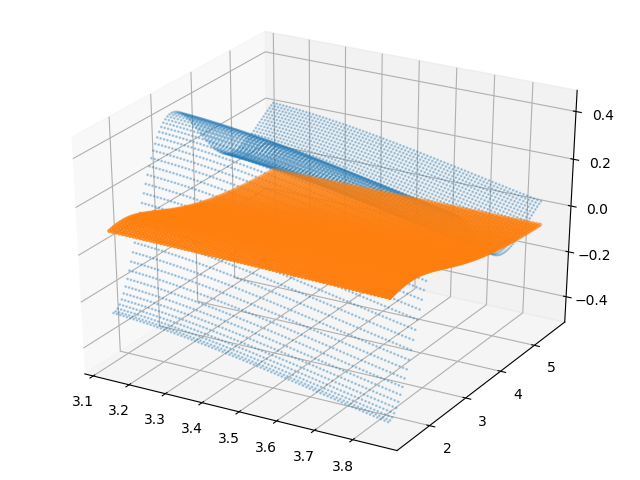
\includegraphics[width=\textwidth]{orig/Sinusoidal-5D-_2D_REMBO.png}
        \caption{Sinusoidal Rembo}
        \label{fig:mouse}
    \end{subfigure}
    \caption{Top-Left: The 2D Sinusoidal-Exponential Function which is embedded in a 5D space.}\label{fig:animals}
\end{figure}

I set the number of restarts to $28$ and number of randomly sampled datapoints to 100.
The active subspace projection matrix is of size $\mathbf{R}^{1\times 5}$, as this is a function that exhibits a strong principal component, but that still attains small perturbations among a different dimension.
One can see very well here, that BORING is able to take into account the small perturbations, at a considerably lower cost than Tripathy would be able to.


% CAMELBACK FUNCTION
\begin{figure}[H]
    \centering
    \begin{subfigure}[b]{0.3\textwidth}
        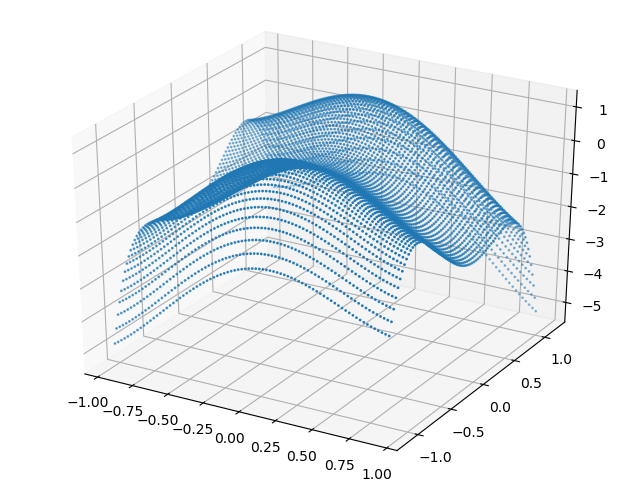
\includegraphics[width=\textwidth]{orig/Camelback-5D-_2D.png}
        \caption{Camelback Original}
        \label{fig:gull}
    \end{subfigure}
    ~ %add desired spacing between images, e. g. ~, \quad, \qquad, \hfill etc. 
      %(or a blank line to force the subfigure onto a new line)
    \begin{subfigure}[b]{0.3\textwidth}
        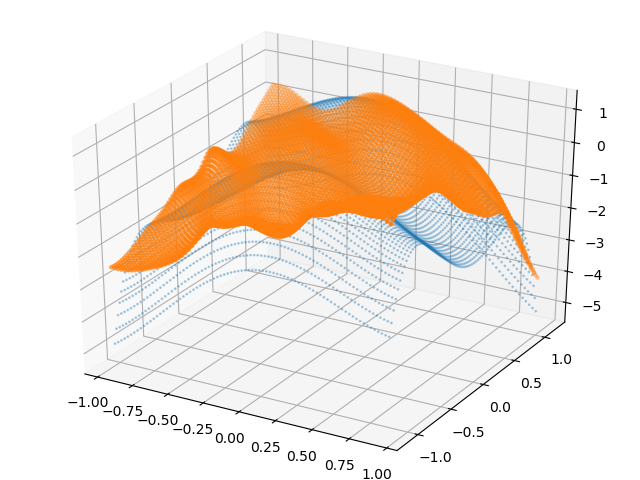
\includegraphics[width=\textwidth]{orig/Camelback-5D-_2D_BORING.png}
        \caption{Camelback Boring}
        \label{fig:tiger}
    \end{subfigure}
        \vskip\baselineskip
 %add desired spacing between images, e. g. ~, \quad, \qquad, \hfill etc. 
    %(or a blank line to force the subfigure onto a new line)
    \begin{subfigure}[b]{0.3\textwidth}
        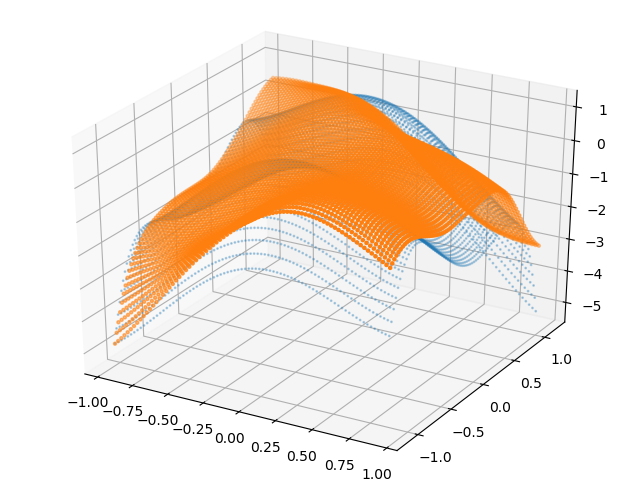
\includegraphics[width=\textwidth]{orig/Camelback-5D-_2D_TRIPATHY.png}
        \caption{Camelback Tripathy}
        \label{fig:mouse}
    \end{subfigure}
        ~ %add desired spacing between images, e. g. ~, \quad, \qquad, \hfill etc. 
    %(or a blank line to force the subfigure onto a new line)
    \begin{subfigure}[b]{0.3\textwidth}
        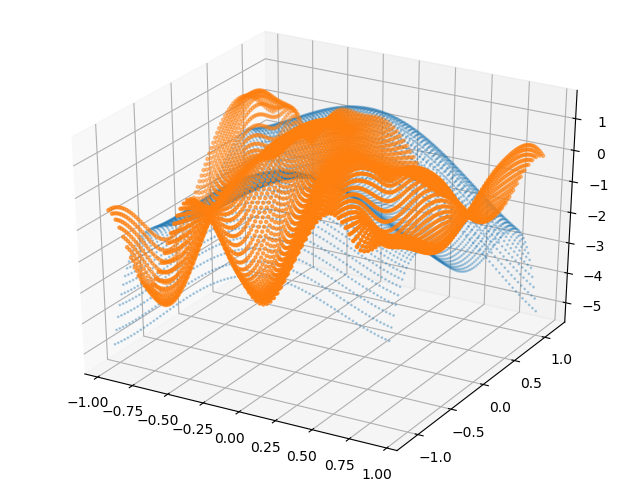
\includegraphics[width=\textwidth]{orig/Camelback-5D-_2D_REMBO.png}
        \caption{Camelback Rembo}
        \label{fig:mouse}
    \end{subfigure}
    \caption{Top-Left: The 2D Camelback Function which is embedded in a 5D space.}\label{fig:animals}
\end{figure}

I set the number of restarts to $28$ and number of randomly sampled datapoints to 100.
The active subspace projection matrix is of size $\mathbf{R}^{2 \times 5}$, as this is a function that lives in a 2D space, and has two strong principal components.
Notice that Tripathy and BORING use the exact same algorithm, as the visualization does not allow to add a third axis. 
In other words, BORING does not add any additional orthogonal vector to the model.
As such, it does not add any additional kernels to the model aswell, and is equivalent to tripathy.


%% Evaluation
%!TEX root = ../thesis.tex
%*******************************************************************************
%****************************** Third Chapter **********************************
%*******************************************************************************
\chapter{Conclusion}

% **************************** Define Graphics Path **************************
\ifpdf
    \graphicspath{{Chapter7/Figs/Raster/}{Chapter7/Figs/PDF/}{Chapter7/Figs/}}
\else
    \graphicspath{{Chapter7/Figs/Vector/}{Chapter7/Figs/}}
\fi


\section{Future work}

Future work could incorporate the synthesis of different methods, including additive GPs and Tripathy's method.
Although Tripathy's method is unbeaten in identifying the active subspace dimension, heuristics could be easily implemented to speed up the calculation time.
To avoid the (small) possibility of identifying a bad subspace, one could make use of the idea of interleaved runs as used in REMBO on Tripathy's method to marginalize this probability even further.
One of the most critical aspects is hyperparameter tuning for the GP models itself.
These can make or break the identification of the subspace.
Choosing bad hyperparameters does not allow us to compare different methods effectively.
In the future, it would be beneficial to address this issue to a stronger extent.
Recalculating the search space for each new point may be too time-consuming, with which REMBO would still be considered state of the art regarding Bayesian Black Box Optimization.
 





%% Conclusion and Future Work
% %!TEX root = ../thesis.tex
%*******************************************************************************
%****************************** Third Chapter **********************************
%*******************************************************************************
\chapter{Conclusion}

% **************************** Define Graphics Path **************************
\ifpdf
    \graphicspath{{Chapter7/Figs/Raster/}{Chapter7/Figs/PDF/}{Chapter7/Figs/}}
\else
    \graphicspath{{Chapter7/Figs/Vector/}{Chapter7/Figs/}}
\fi


\section{Future work}

Future work could incorporate the synthesis of different methods, including additive GPs and Tripathy's method.
Although Tripathy's method is unbeaten in identifying the active subspace dimension, heuristics could be easily implemented to speed up the calculation time.
To avoid the (small) possibility of identifying a bad subspace, one could make use of the idea of interleaved runs as used in REMBO on Tripathy's method to marginalize this probability even further.
One of the most critical aspects is hyperparameter tuning for the GP models itself.
These can make or break the identification of the subspace.
Choosing bad hyperparameters does not allow us to compare different methods effectively.
In the future, it would be beneficial to address this issue to a stronger extent.
Recalculating the search space for each new point may be too time-consuming, with which REMBO would still be considered state of the art regarding Bayesian Black Box Optimization.
 







% ********************************** Back Matter *******************************
% Backmatter should be commented out, if you are using appendices after References
%\backmatter

% ********************************** Bibliography ******************************
\begin{spacing}{0.9}

% To use the conventional natbib style referencing
% Bibliography style previews: http://nodonn.tipido.net/bibstyle.php
% Reference styles: http://sites.stat.psu.edu/~surajit/present/bib.htm

\bibliographystyle{apalike}
%\bibliographystyle{unsrt} % Use for unsorted references  
%\bibliographystyle{plainnat} % use this to have URLs listed in References
\cleardoublepage
\bibliography{References/references} % Path to your References.bib file


% If you would like to use BibLaTeX for your references, pass `custombib' as
% an option in the document class. The location of 'reference.bib' should be
% specified in the preamble.tex file in the custombib section.
% Comment out the lines related to natbib above and uncomment the following line.

%\printbibliography[heading=bibintoc, title={References}]


\end{spacing}

% ********************************** Appendices ********************************

\begin{appendices} % Using appendices environment for more functunality

%!TEX root = ../thesis.tex
% ******************************* Thesis Appendix A ****************************
\chapter{How to install \LaTeX} 

\section*{Mac OS X}
\subsection*{MacTeX - \TeX~ distribution}
\begin{enumerate}
\item	Download the file from\\
\href{https://www.tug.org/mactex/}{https://www.tug.org/mactex/}
\item	Extract and double click to run the installer. It does the entire configuration, sit back and relax.
\end{enumerate}

\end{appendices}

% *************************************** Index ********************************
\printthesisindex % If index is present

\end{document}
